\documentclass{article}
\usepackage[utf8]{inputenc}

\usepackage{amsmath}
\usepackage{amssymb}
\usepackage{amsthm}
\usepackage{graphicx}
\usepackage{array}
%
\theoremstyle{definition}
\newtheorem{theorem}{Theorem}
\newtheorem{definition}{Definition}
\newtheorem*{remark}{Remark}
\newtheorem*{notation}{Notation}
\newtheorem{construction}{Construction}

\title{Statistical Analysis of Permutations}
\author{Jojo W. Whaley Aboaf, Martin T. Wells}
\date{February 2021}

\begin{document}
\maketitle
\tableofcontents
\section{Motivation}
We are interested in determining if there is nationality bias in international surf competition. One can measure bias in many ways, however, not all of them may be appropriate, robust, or informative. So our focus is on the which methodologies are most appropriate and why.


Our goal is to determine if judges have a tendency to give higher scores to surfers from their home country when compared to judges with a different home country.

For any given ride, there is one surfer. The surfer has a nationality. Each judge on the panel has a nationality. So we can identify two subsets of the panel:

Matching Judges = {judge on Panel | judge nationality = surfer nationality }
Non-Matching Judges = {judge on Panel | judge nationality != surfer nationality}

A judge in Matching Judges is called a match. A judge in Non-Matching Judges is called a non-match. This may seem to be a fairly straightforward statistical problem where testing for differences in means or rank tests may be applied. (These come with some dissatisfactions though: wave scores are certainly not determined by parametric distributions of judge countries (they are functions of wave quality and surfer performance), we can only carry out rank tests on an individual wave because that is the only level at which scores are I.I.D, going up to heat level i.e. multiple waves gives lots of variability from wave to wave and I.I.D. assumptions would be ridiculous.)

(In a way) we can answer our question by labelling each judge on the panel for a wave using $M :=\{$Match, Non-Match$\}$, and analyzing the frequencies of arrangements of M: [Match, Non-Match], [Non-Match, Match].

However, in analyzing our data from the "Match or Non-match" standpoint we have made the overarching assumption that the  surfer's country is immaterial, which is particularly concerning because it is the single factor determining if a judge is a match or non-match. And in this viewpoint "surfer A is from Brazil and Judge 3 is from Brazil " vs. "surfer B is from Australia and Judge 2 is from Australia". Precisely, the assumption is that, nationality bias is uniform over all of the countries. 

To analyze the orders of judges by nationality, it suffices to analyze the orderings of the set $C := \{AUS, BRA, FRA, \dots, ZAF\}$, which is the set of all nationalities of judges who scored any wave from 2017 to 2019.

\section{Introduction}
The World Surf League (WSL) is the most prominent organizer of international surf competitions.  Each year the WSL organizes a variety of ”tours” which include Men's and Women's versions of Big Wave events, the ”Longboard Tour”, the ”Qualifying Series”, and the ”Championship Tour” (CT)

 Does nationality influence the World Surf League Championship Tour? If so, how?, to what degree?, and does this vary depending on nationality?

\subsection{Format}
Each  year,  the  32  highest  ranked  (short board)  surfers  are  invited  to  participate  in  the”Championship Tour” (CT), which consists of 11 surf competitions in 7 different countries.Each competition has 7 rounds, each consisting of 1 to 16 heats, and each heat has 2 to 3surfers.  Within a heat, a surfer may attempt to ride any number of waves, but their final heat score is the sum of their two highest scoring waves.  The surfer with the highest heat score places 1st in the heat, the surfer with the next highest heat score places 2nd in the heat.In some rounds, heats consist of 3 surfers, in which case the surfer with the third highest heat score will place 3rd in the heat.

\subsection{Data}
The World Surf League (WSL) holds a variety of tours or series' at the professional or amateur level (similar to how the MLB organizes A, AA, and AAA baseball). A "tour" or "series" is a sequence of events. Tours have seasons that typically last no more than 365 days and they tend to be contained within one calendar year (i.e. there is a 2019 season of a tour).

We collected some rich data on the 2017, 2018, and 2019 seasons of the Men's Championship Tour (CT). This is the highest level of competitive short board surfing in the world. Each season typically consists of 10 or 11 surf competitions, which are called "events". The format of an event has changed throughout our sample, but they are fairly similar. An event consists of 7 or 8 rounds, and within each round there are some number of heats. A "heat" is the level where direct competition between athletes takes place. Typically, there are 2 or 3 surfers in a heat and the duration is between 22 and 35 minutes. During a heat, a surfer may attempt to ride any number of waves. Anytime a surfer rides a wave, they receive a non-zero score determined by the scores of a judging panel. There are 5 judges on a panel for any given heat. They are visually separated and do not discuss scores. When a surfer takes a wave, they each observe the ride and write down a score which is some number between 0.1 and 10.0 and it is precise up to the tenths place. The highest and lowest scores given by the panel are dropped, and the surfer receives the mean of the 3 remaining scores for their ride, this is called the "wave score". These are rounded to 2 digits. At any given point in a heat, a surfer has a "heat score", which is the sum of their two highest scores, and simply the sum of their scores if they have surfed 0, 1, or 2 waves. When the time allocated for a heat elapses, a horn will sound, and the surfer with the highest heat score is awarded first place, the surfer with the second highest score is awarded second, and so on, if there are more surfers. The result of finishing a heat in a particular place depends on the round.  Each round has a rule that determines which surfers advance, and what (round,heat) they advance to.  Surfers that do not advance ”exit” the event and are given some number of points. (The longer a surfer stays in an event, the more points they are allocated at an exit). The 2019 event format is depicted below.
THOUGHT: Maybe i should add number of points to the exists.
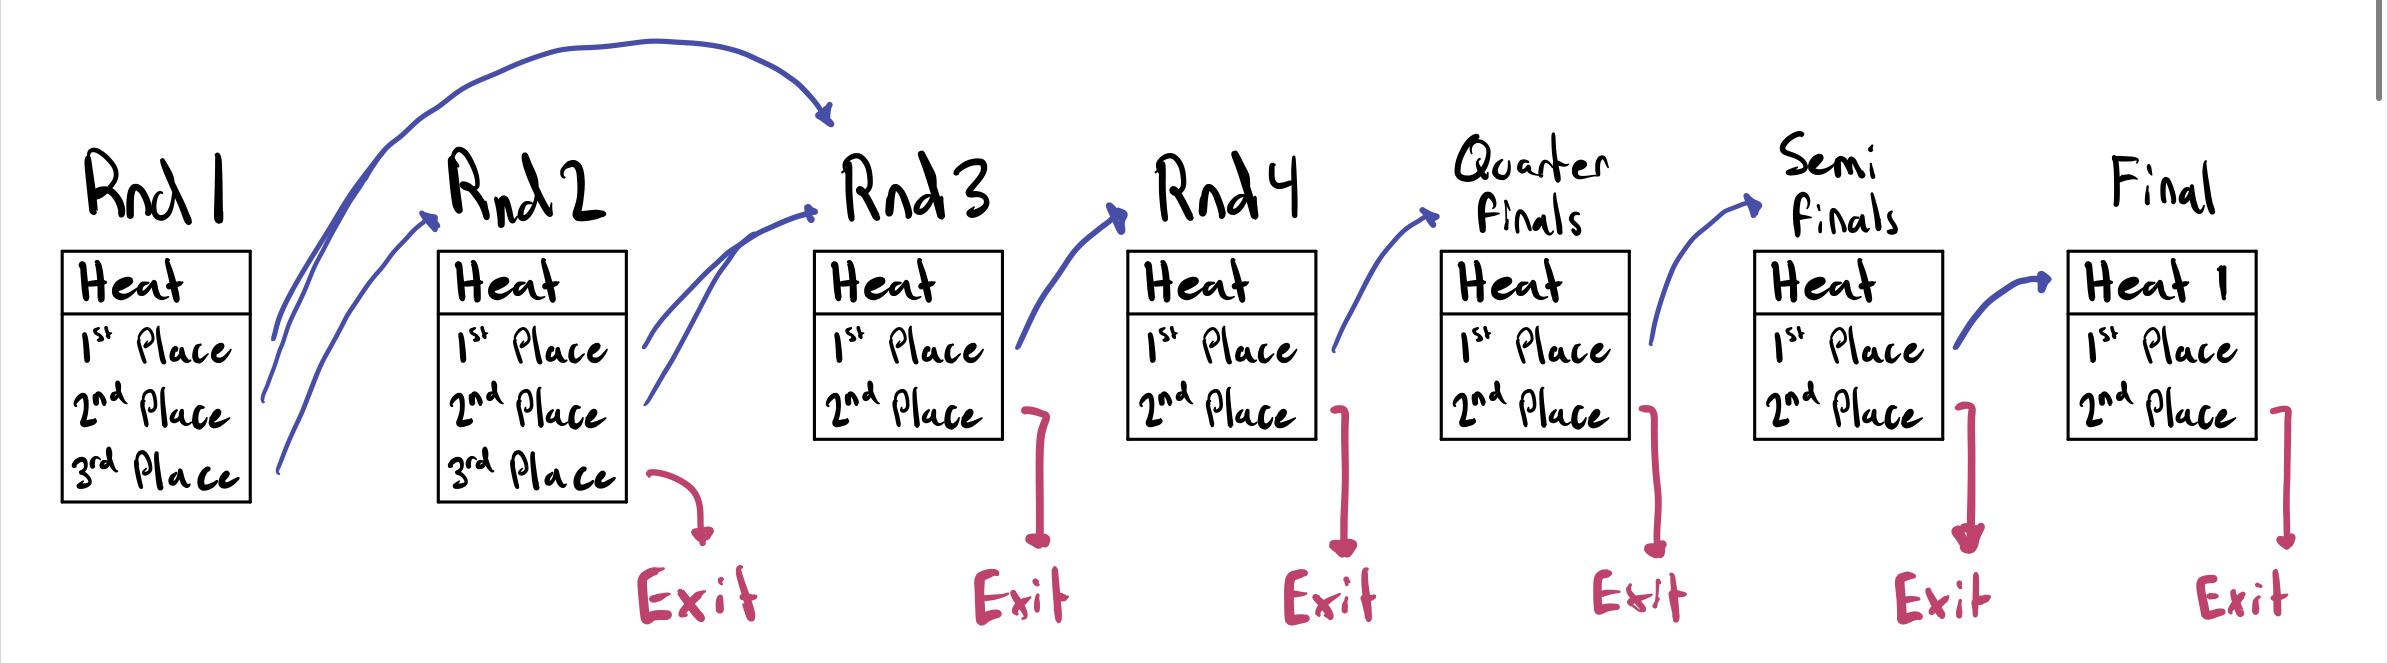
\includegraphics[width=\textwidth]{./src/visuals/2019EvtFormat.jpeg}

\subsubsection{Data Collection}
\begin{center}
\begin{tabular}{|c|c|c|c|c|c| }
\multicolumn{2}{c}{} & \multicolumn{2}{c}{Origins Listed} & \multicolumn{2}{c}{Sub Scores listed} \\
\hline
Year & Waves & 0 Origins & 5 Origins & 3 Sub Scores & 5 Sub Scores \\ 
\hline
2017 & 7328 & 5210 & 2118  & 299 & 7029  \\
2018 & 6639 & 336 & 6303  & 0 & 6639  \\
2019 & 7648 & 79 & 7569  & 0 & 7648 \\
\hline
All & 21615 & 5625 & 15990 & 299 & 21316 \\
\hline
\end{tabular}
\end{center}

\subsubsection{Random Variables}
Simply put, we collected some information on a real world random process. The source of this information is www.worldsurfleague.com .

\section{The Simple Approach}
Our goal is to determine if judges have a tendency to give higher scores to surfers that share their same nationality.
The straight forward approach is to test the differences in means between judges with the same nationality as the surfer and those with a different nationality. So we perform a hypothesis test where our hypotheses are:
\[ H_0: \mu_M  - \mu_{\neg M} = 0  \quad H_1: \mu_M -\mu_{\neg M} \neq 0 \]
And the test statistic is $ t = \frac{\bar{x}}{s/\sqrt{N}} $. Note that we are performing a one sample t-test on a series of data $(x_i)_{i=1}^N$ where $x_i := \mu_{M,i}  - \mu_{\neg M,i}$.  We'd like to call a panel for a wave our "statistical unit". This would be a lie. Not every panel is included in these tests because some panels have 0 Judges from the same country as the surfer riding the wave. Which means the difference in means between Matching judges and Non-Matching judges looks like:
\[\frac{\sum_{j \in \text{Matching Judges}} score(j) }{|\{Matching Judges\}|} - \frac{\sum_{j \in\text{Non-Matching Judges}} score(j) }{|\{Non-Matching Judges\}|} = \frac{0}{0} - \frac{\sum_{j \in\text{Non-Matching Judges}} score(j) }{|\{Non-Matching Judges\}} \]
This is undefined. Nonetheless, we are only interested in the difference in means when there is a match between at least one judge's nationality and the surfer's nationality. Carrying out this test, we obtain a t-value around 6.71160420326186
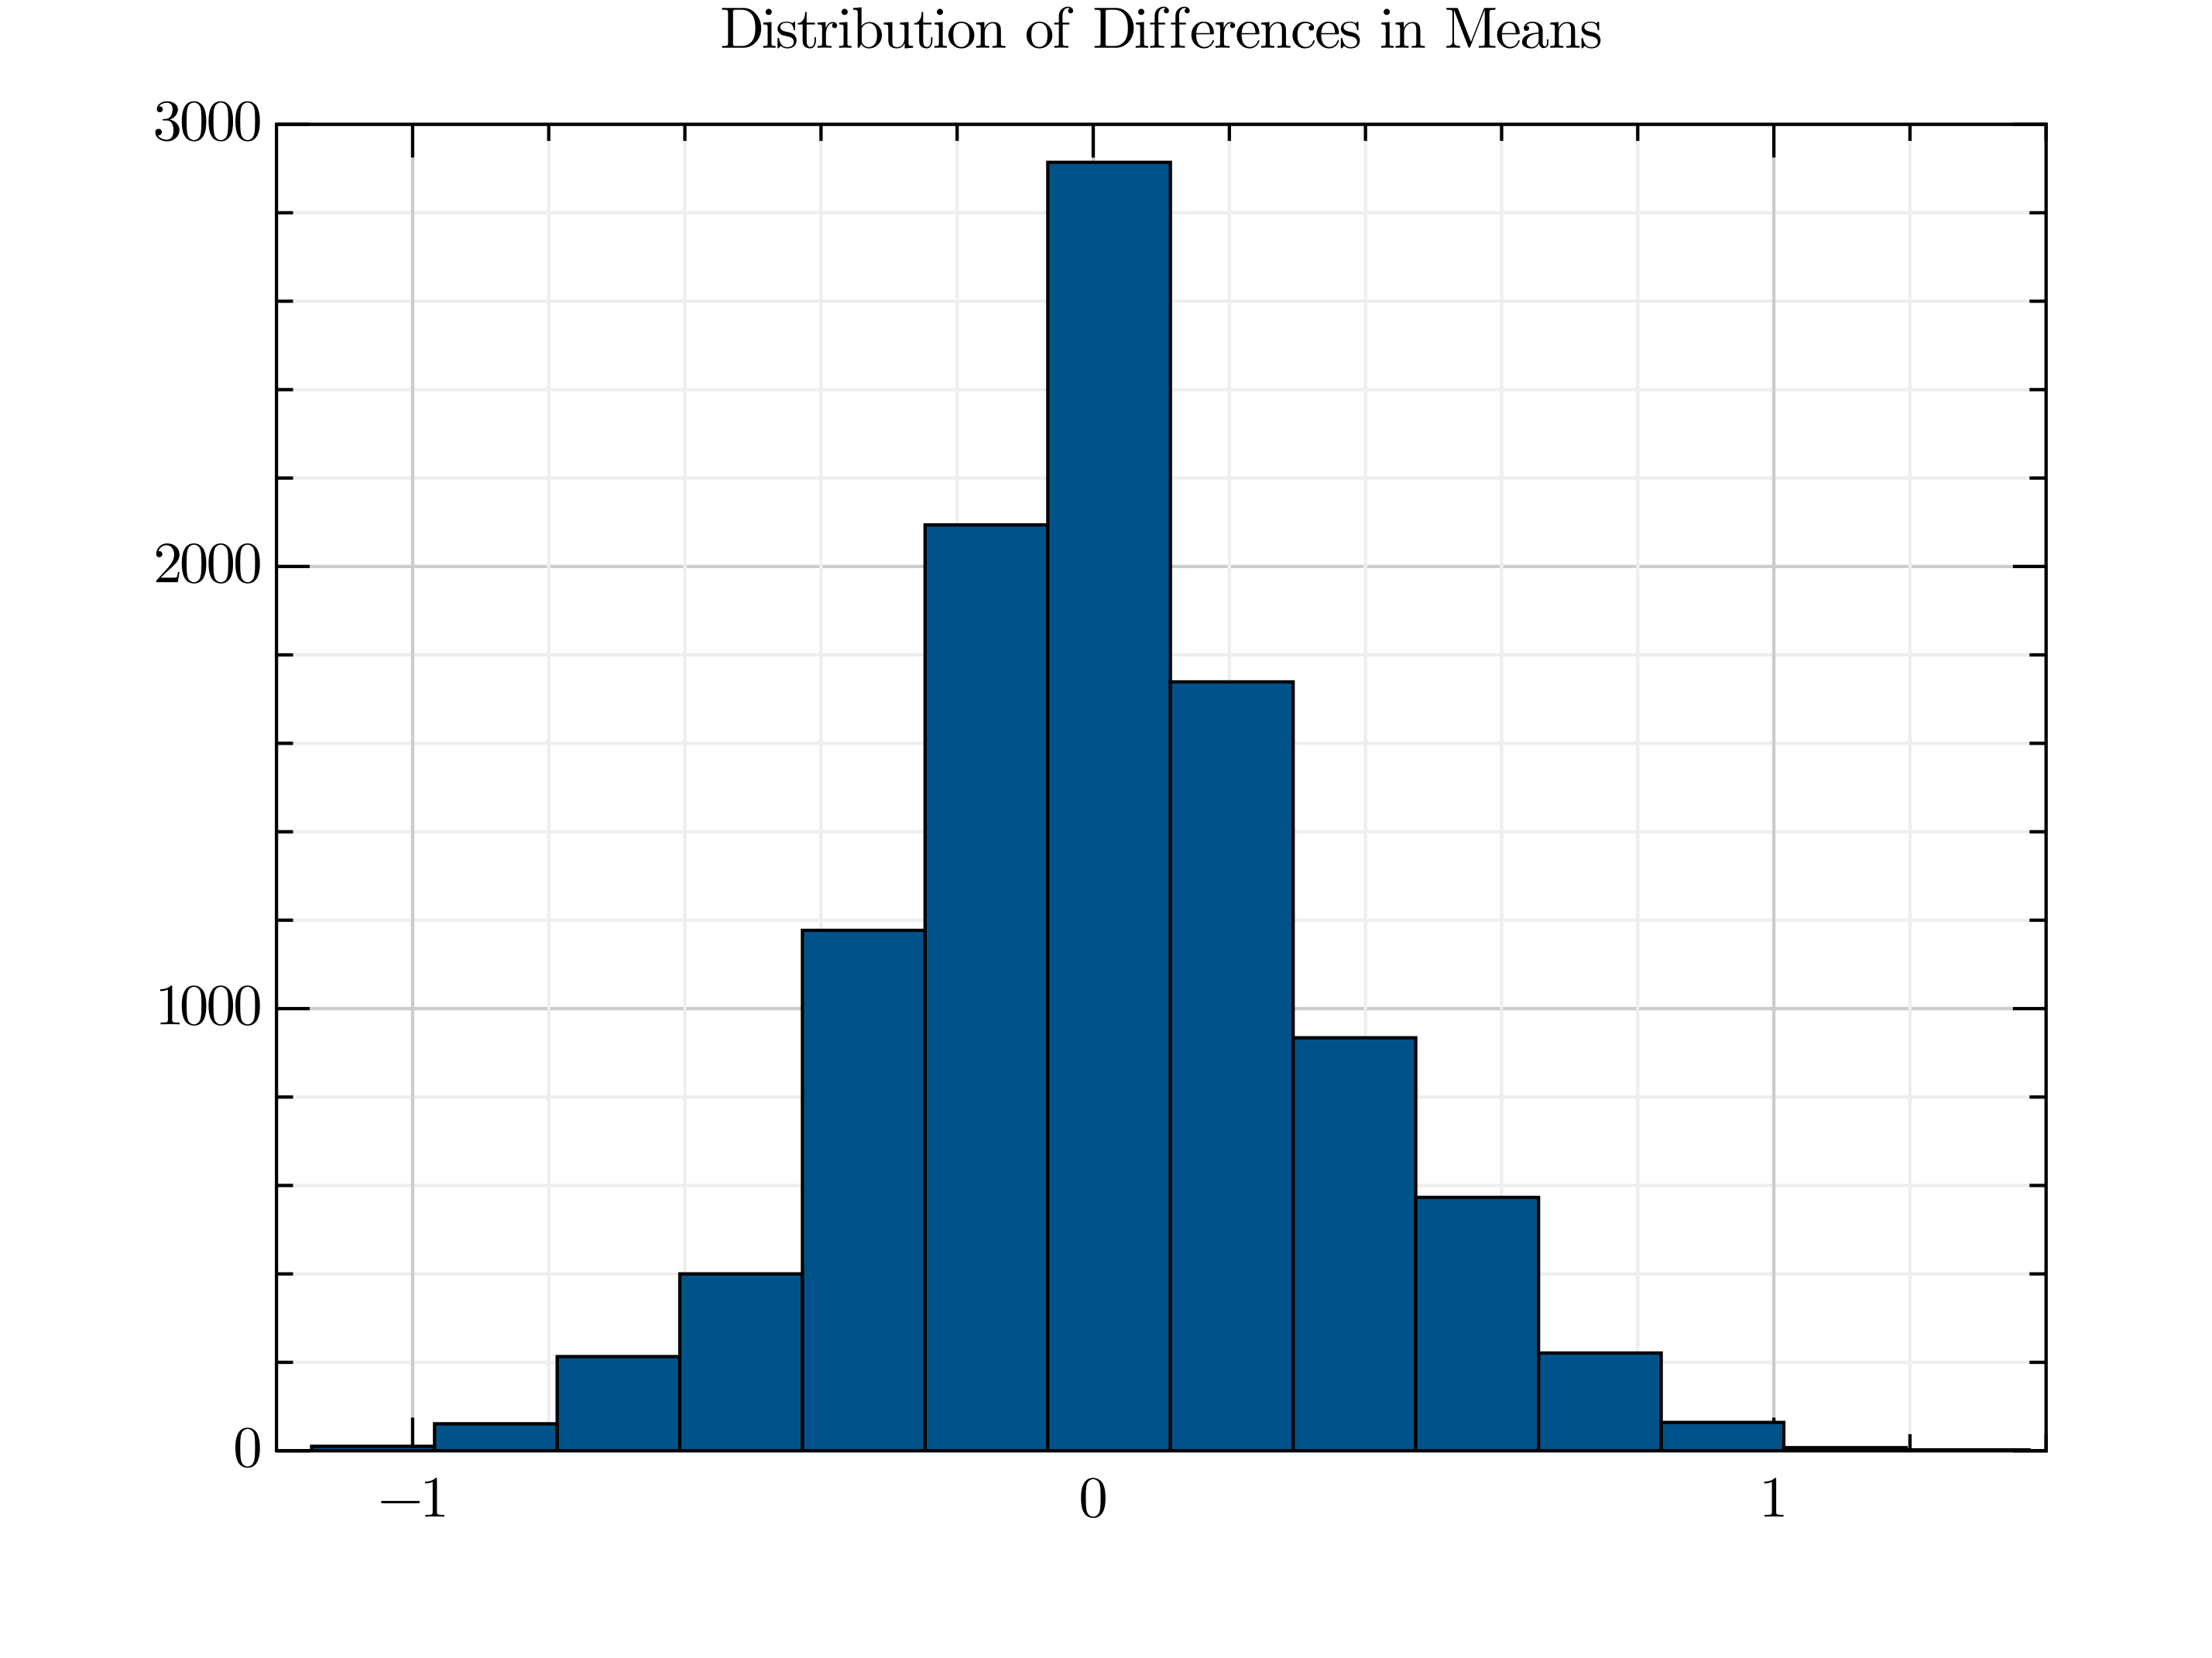
\includegraphics[width=\textwidth]{./src/visuals/DistOfDiffInMeans.png}

Note there is no Diff In Means for ESP because there are 0 waves where AthOrig = ESP and ESP in Judge Origs

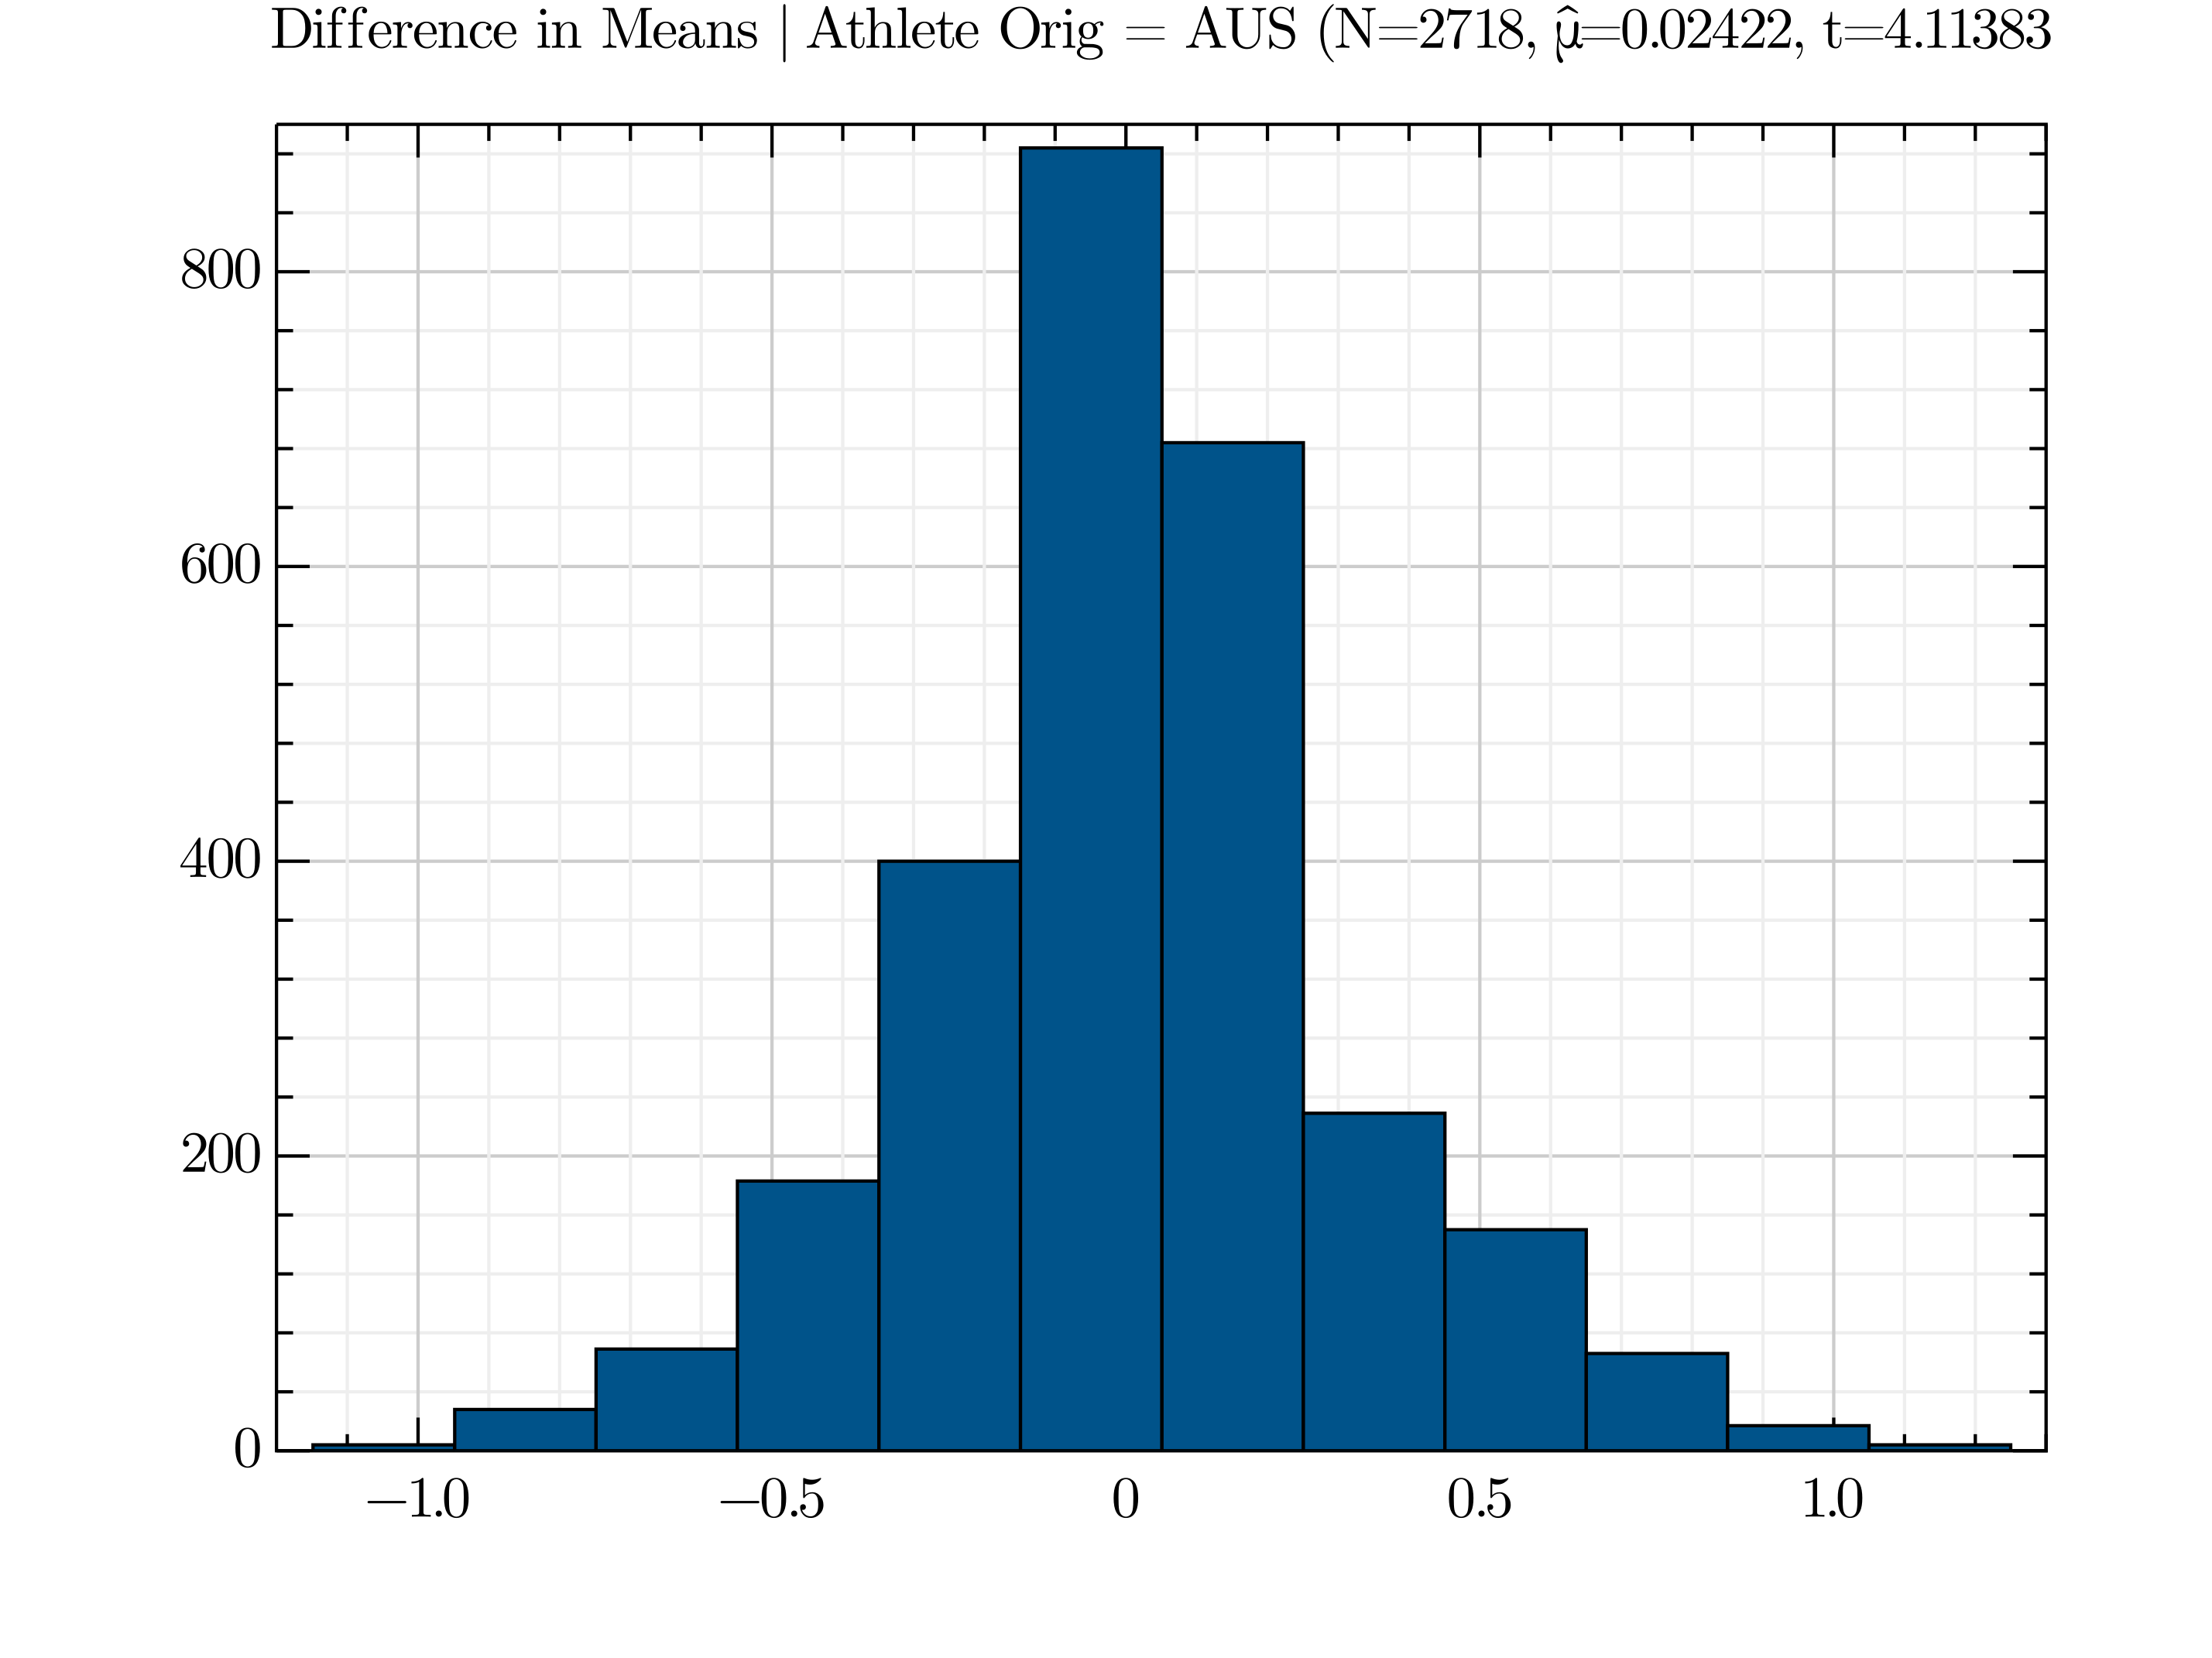
\includegraphics[width=8cm]{./src/visuals/DistOfDiffInMeansForAUS.png}
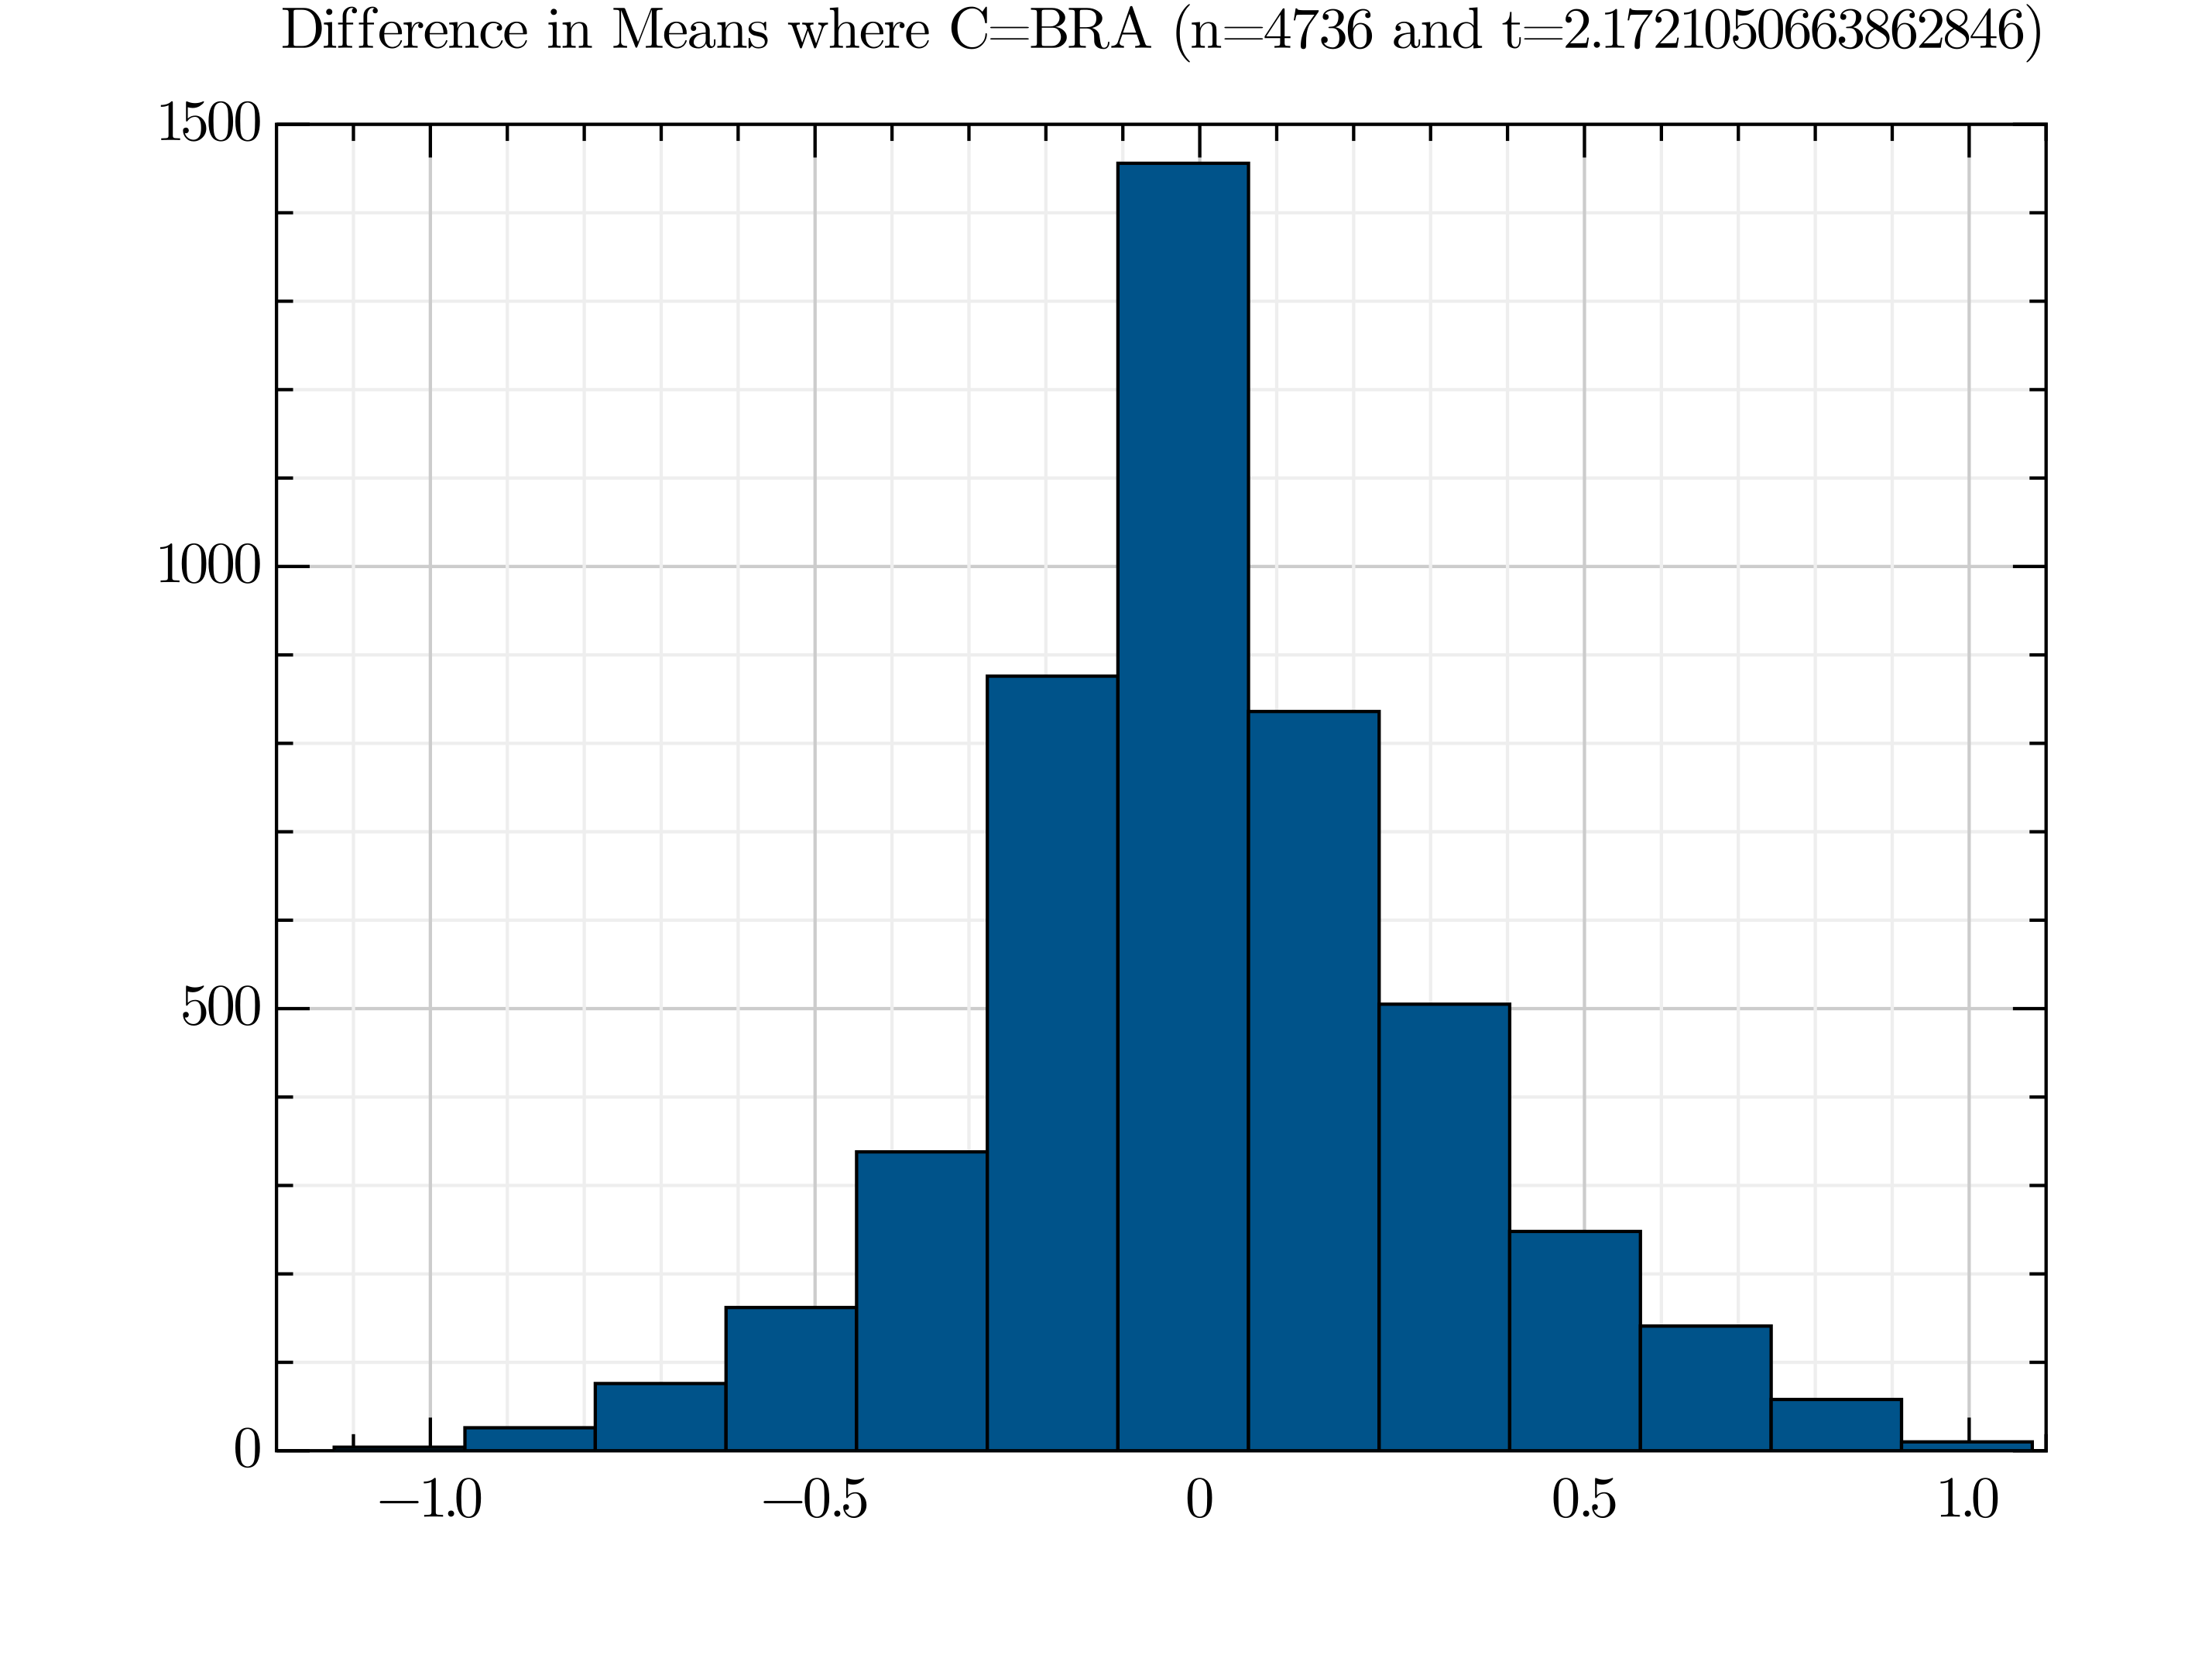
\includegraphics[width=8cm]{./src/visuals/DistOfDiffInMeansForBRA.png}
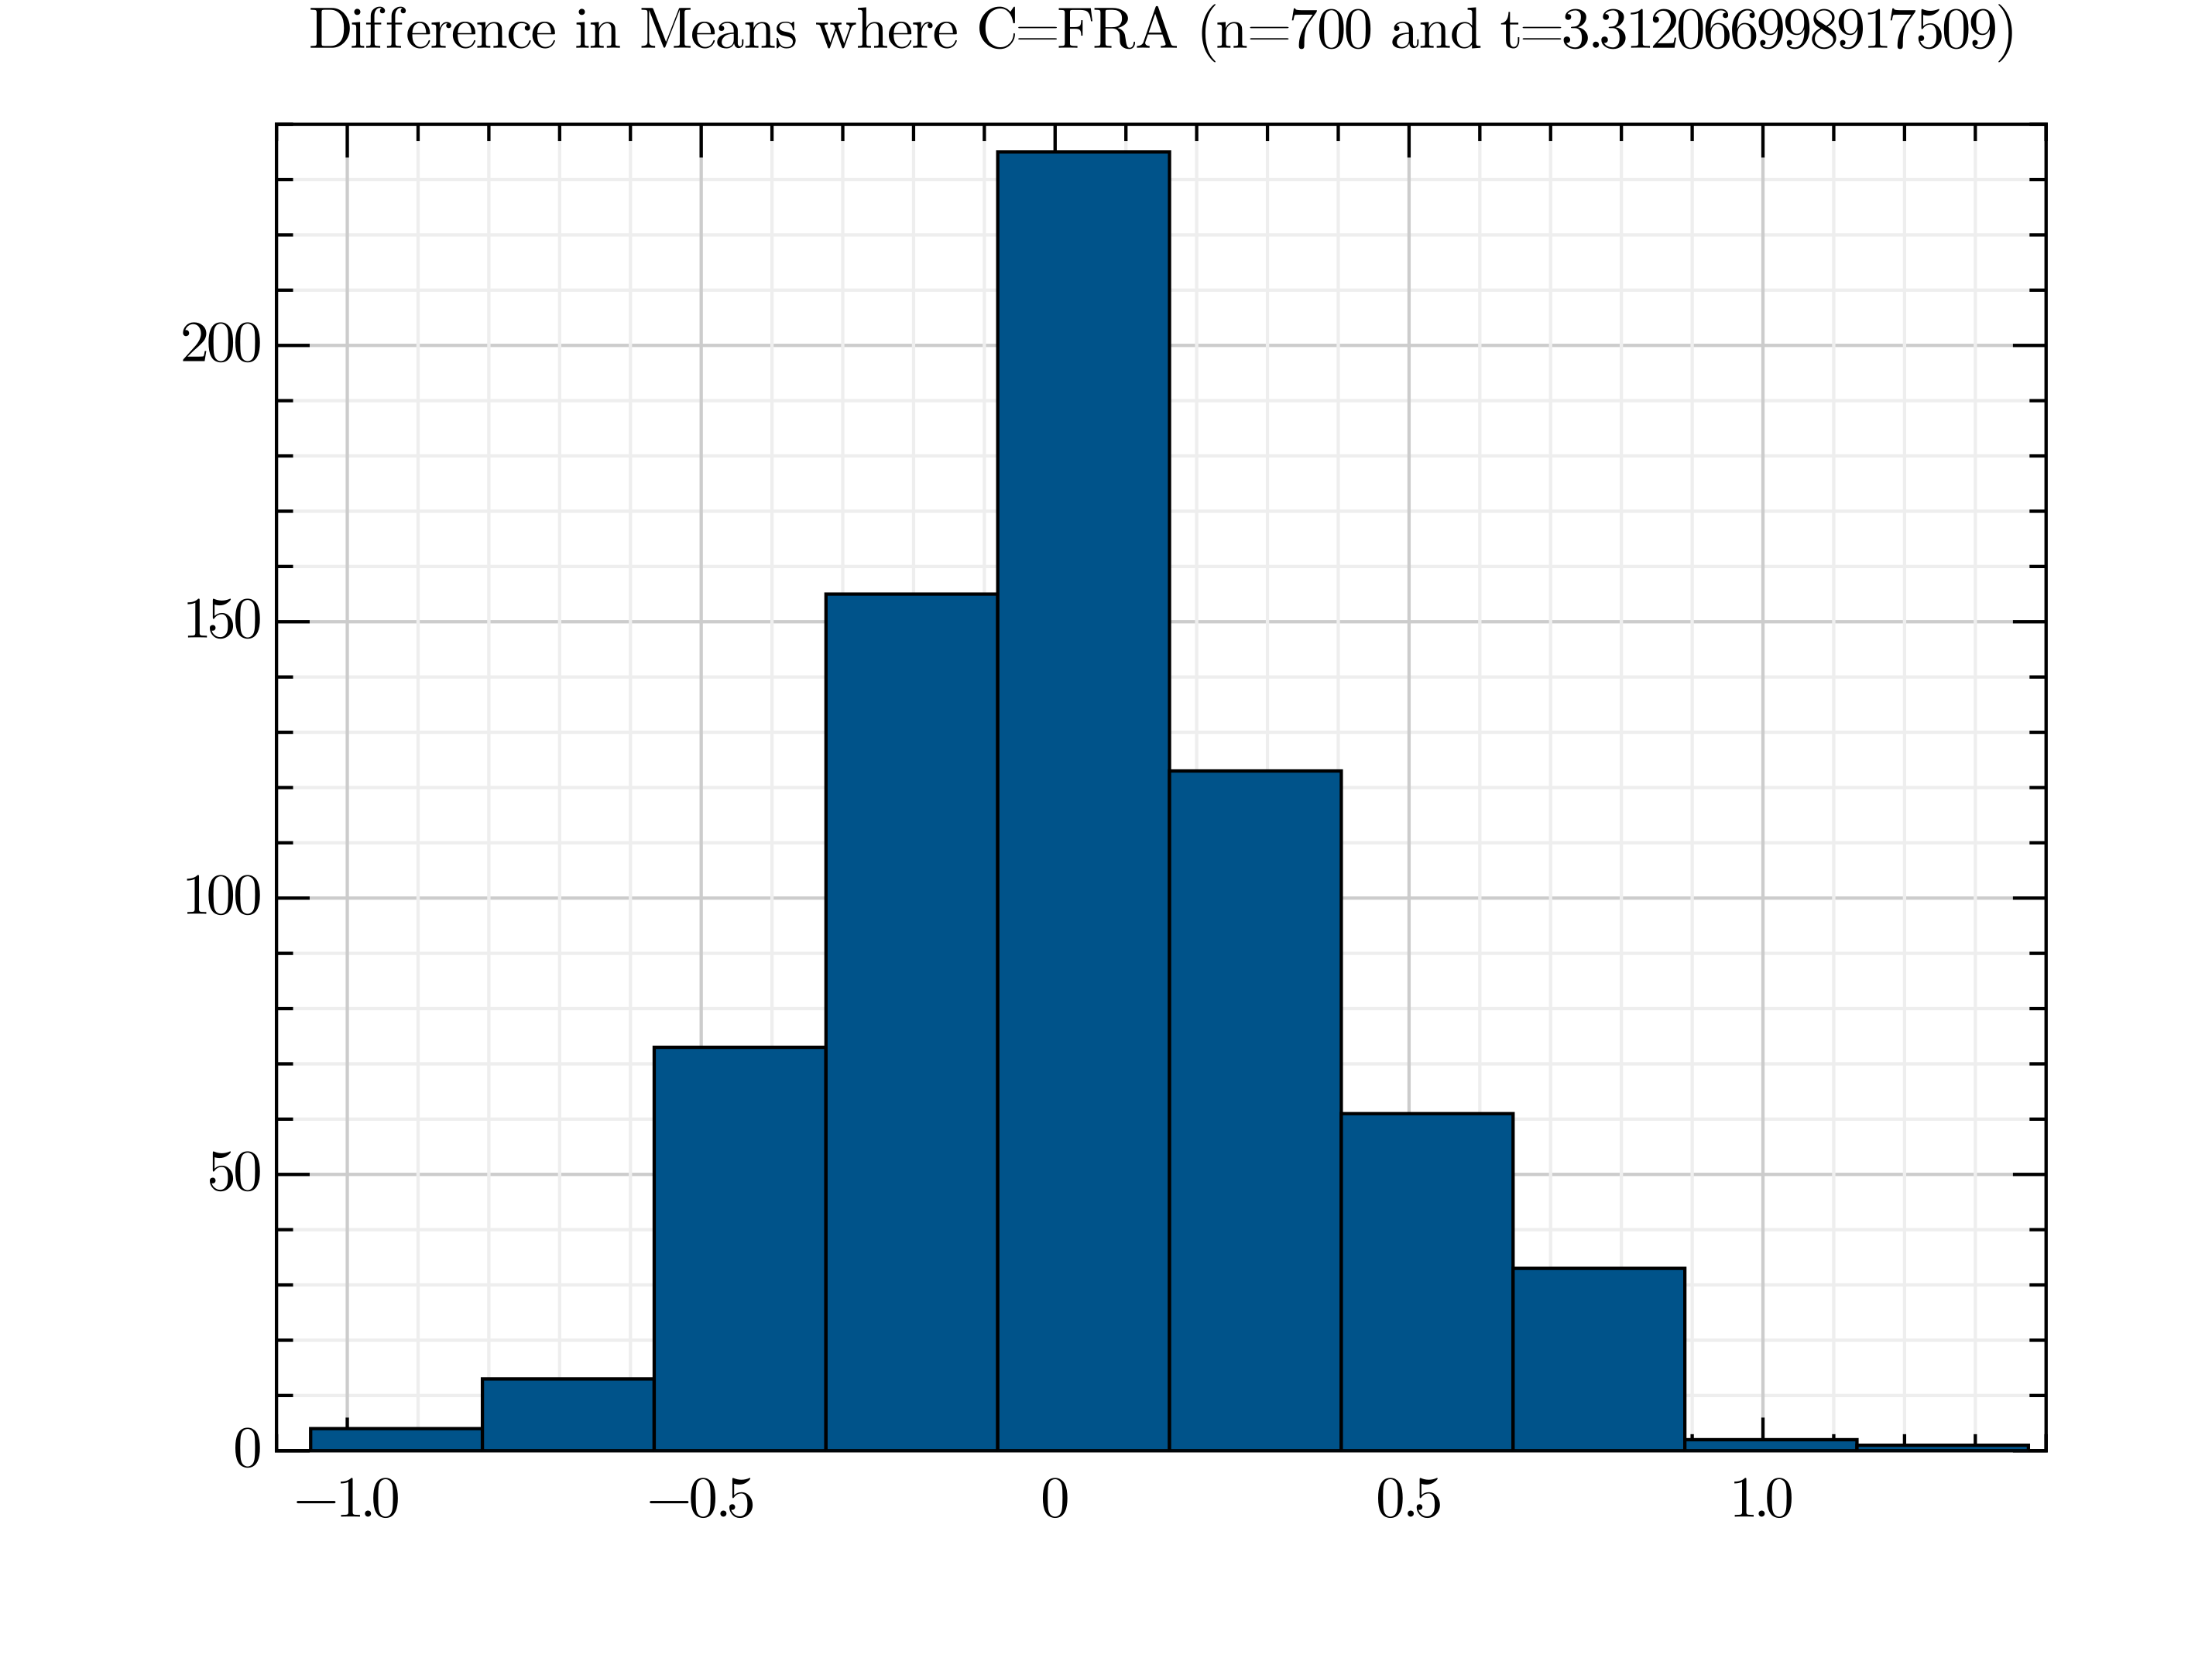
\includegraphics[width=8cm]{./src/visuals/DistOfDiffInMeansForFRA.png}
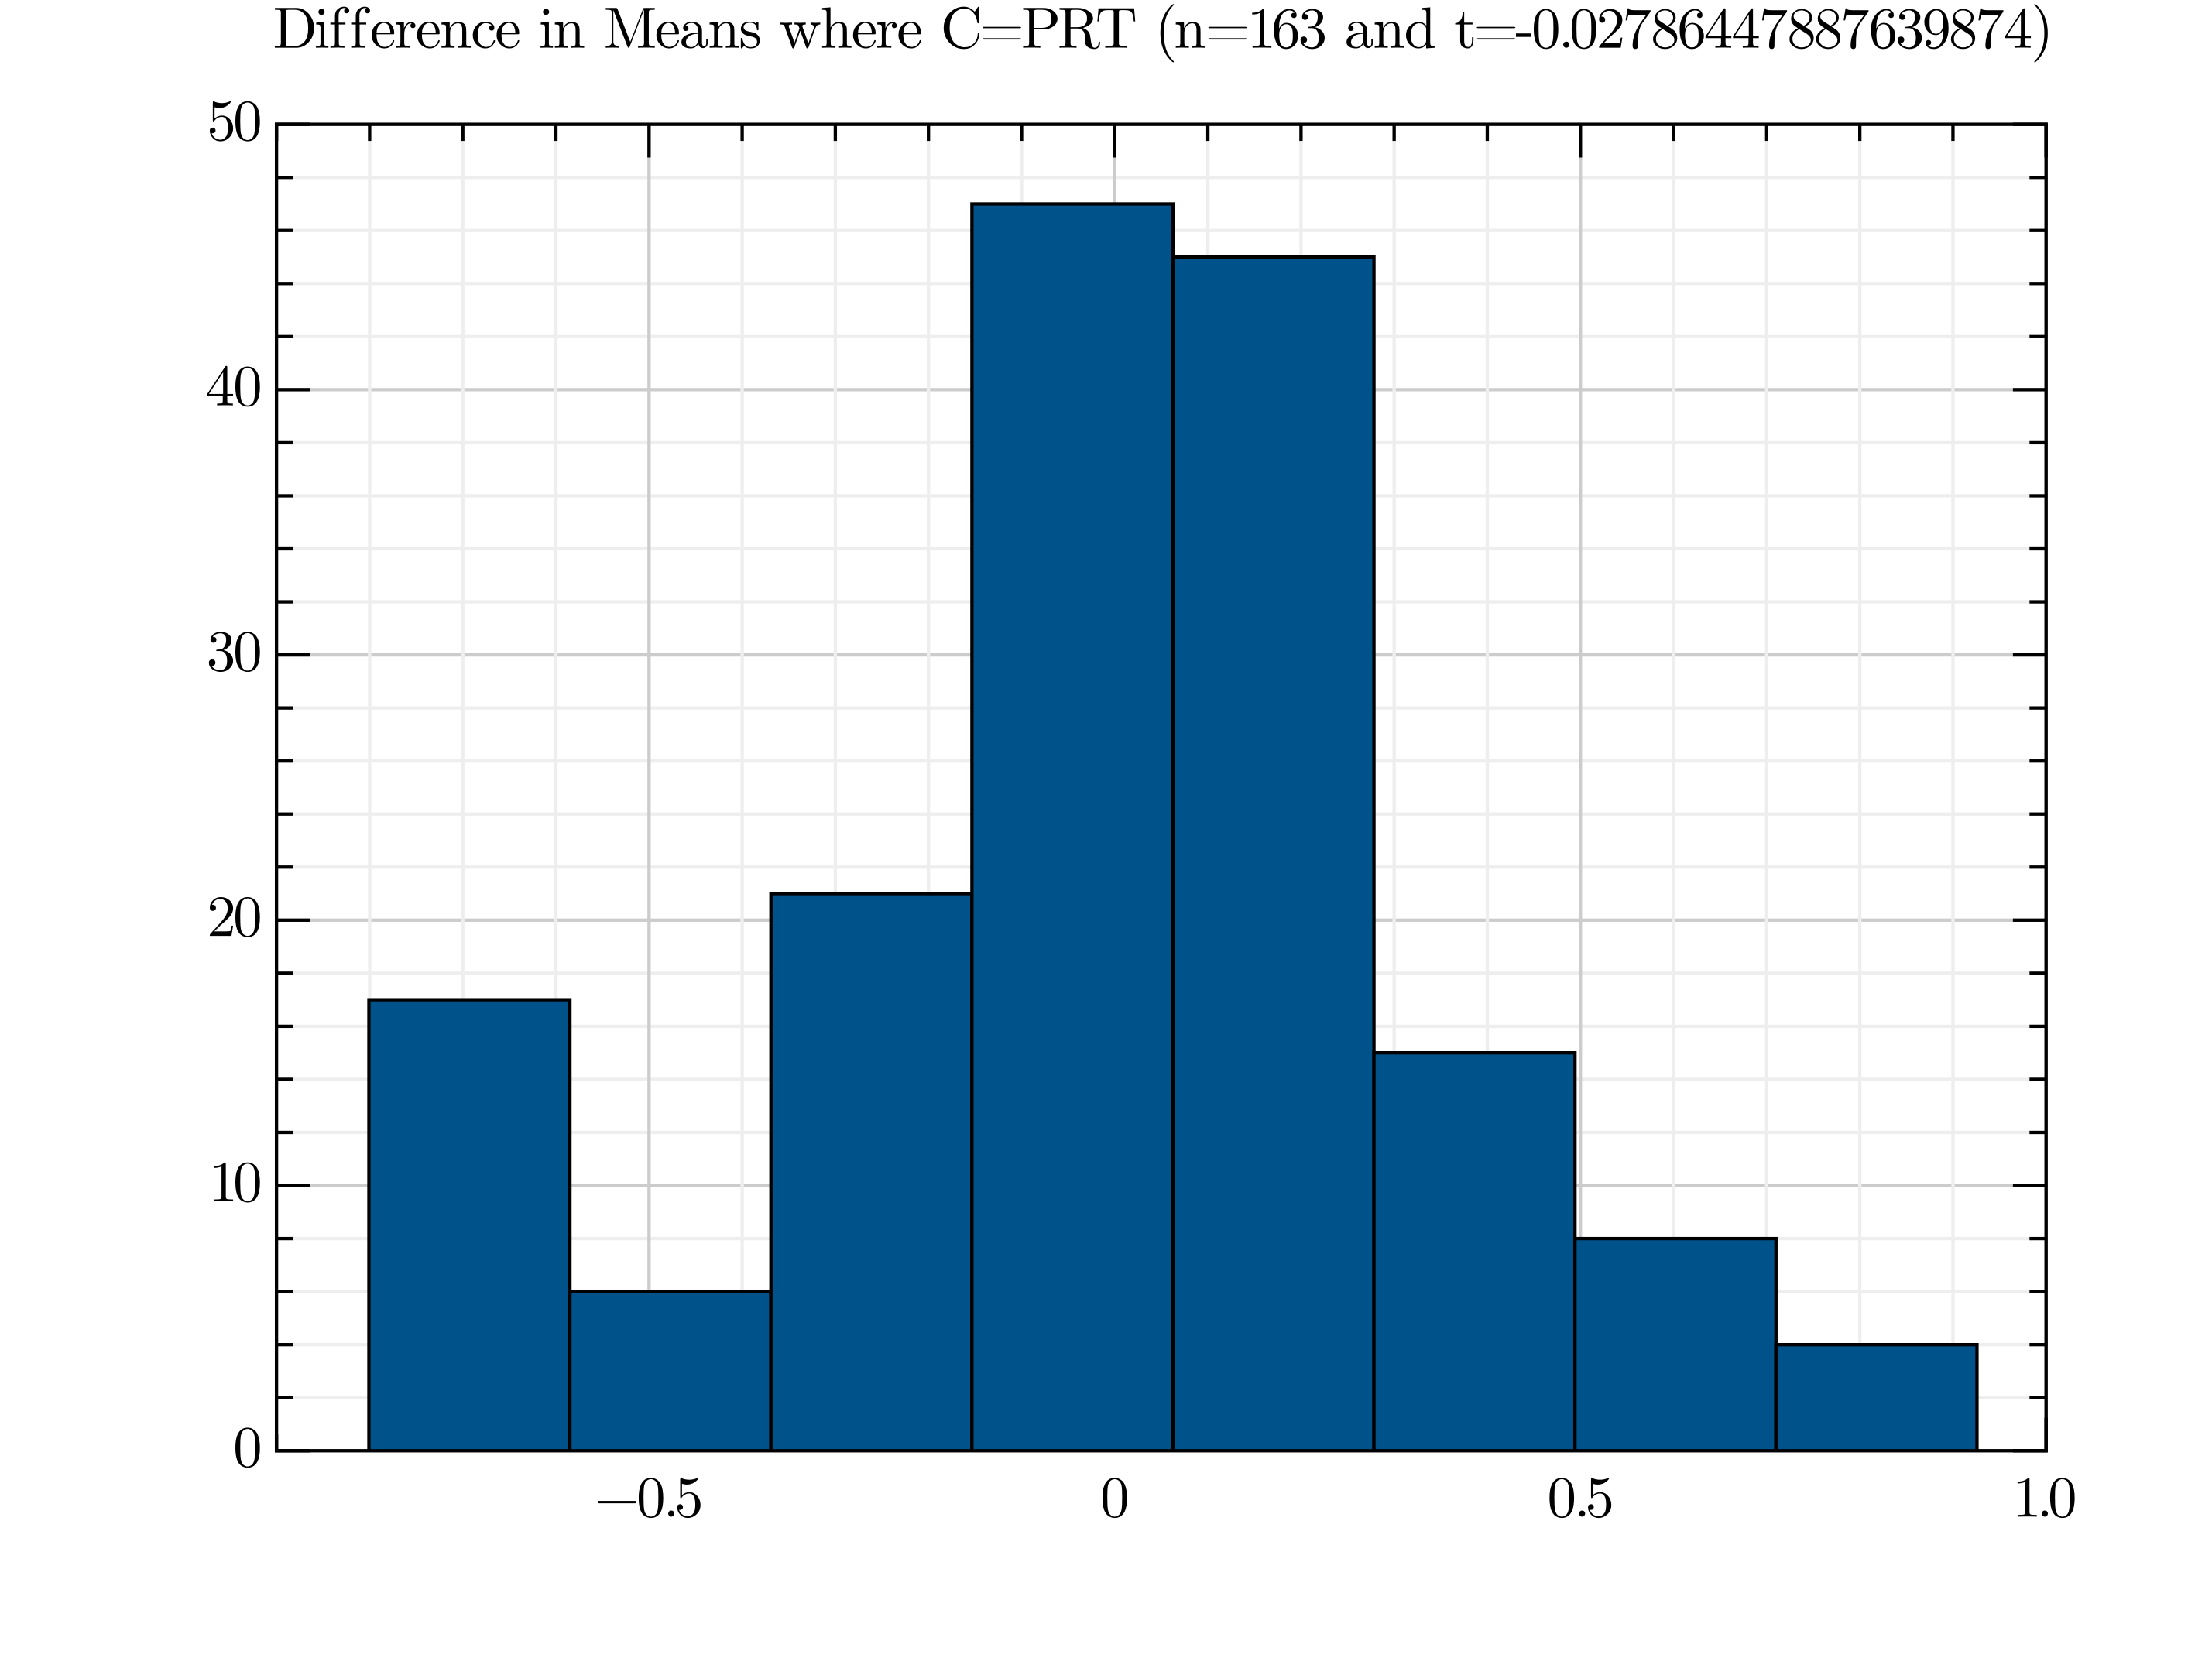
\includegraphics[width=8cm]{./src/visuals/DistOfDiffInMeansForPRT.png}
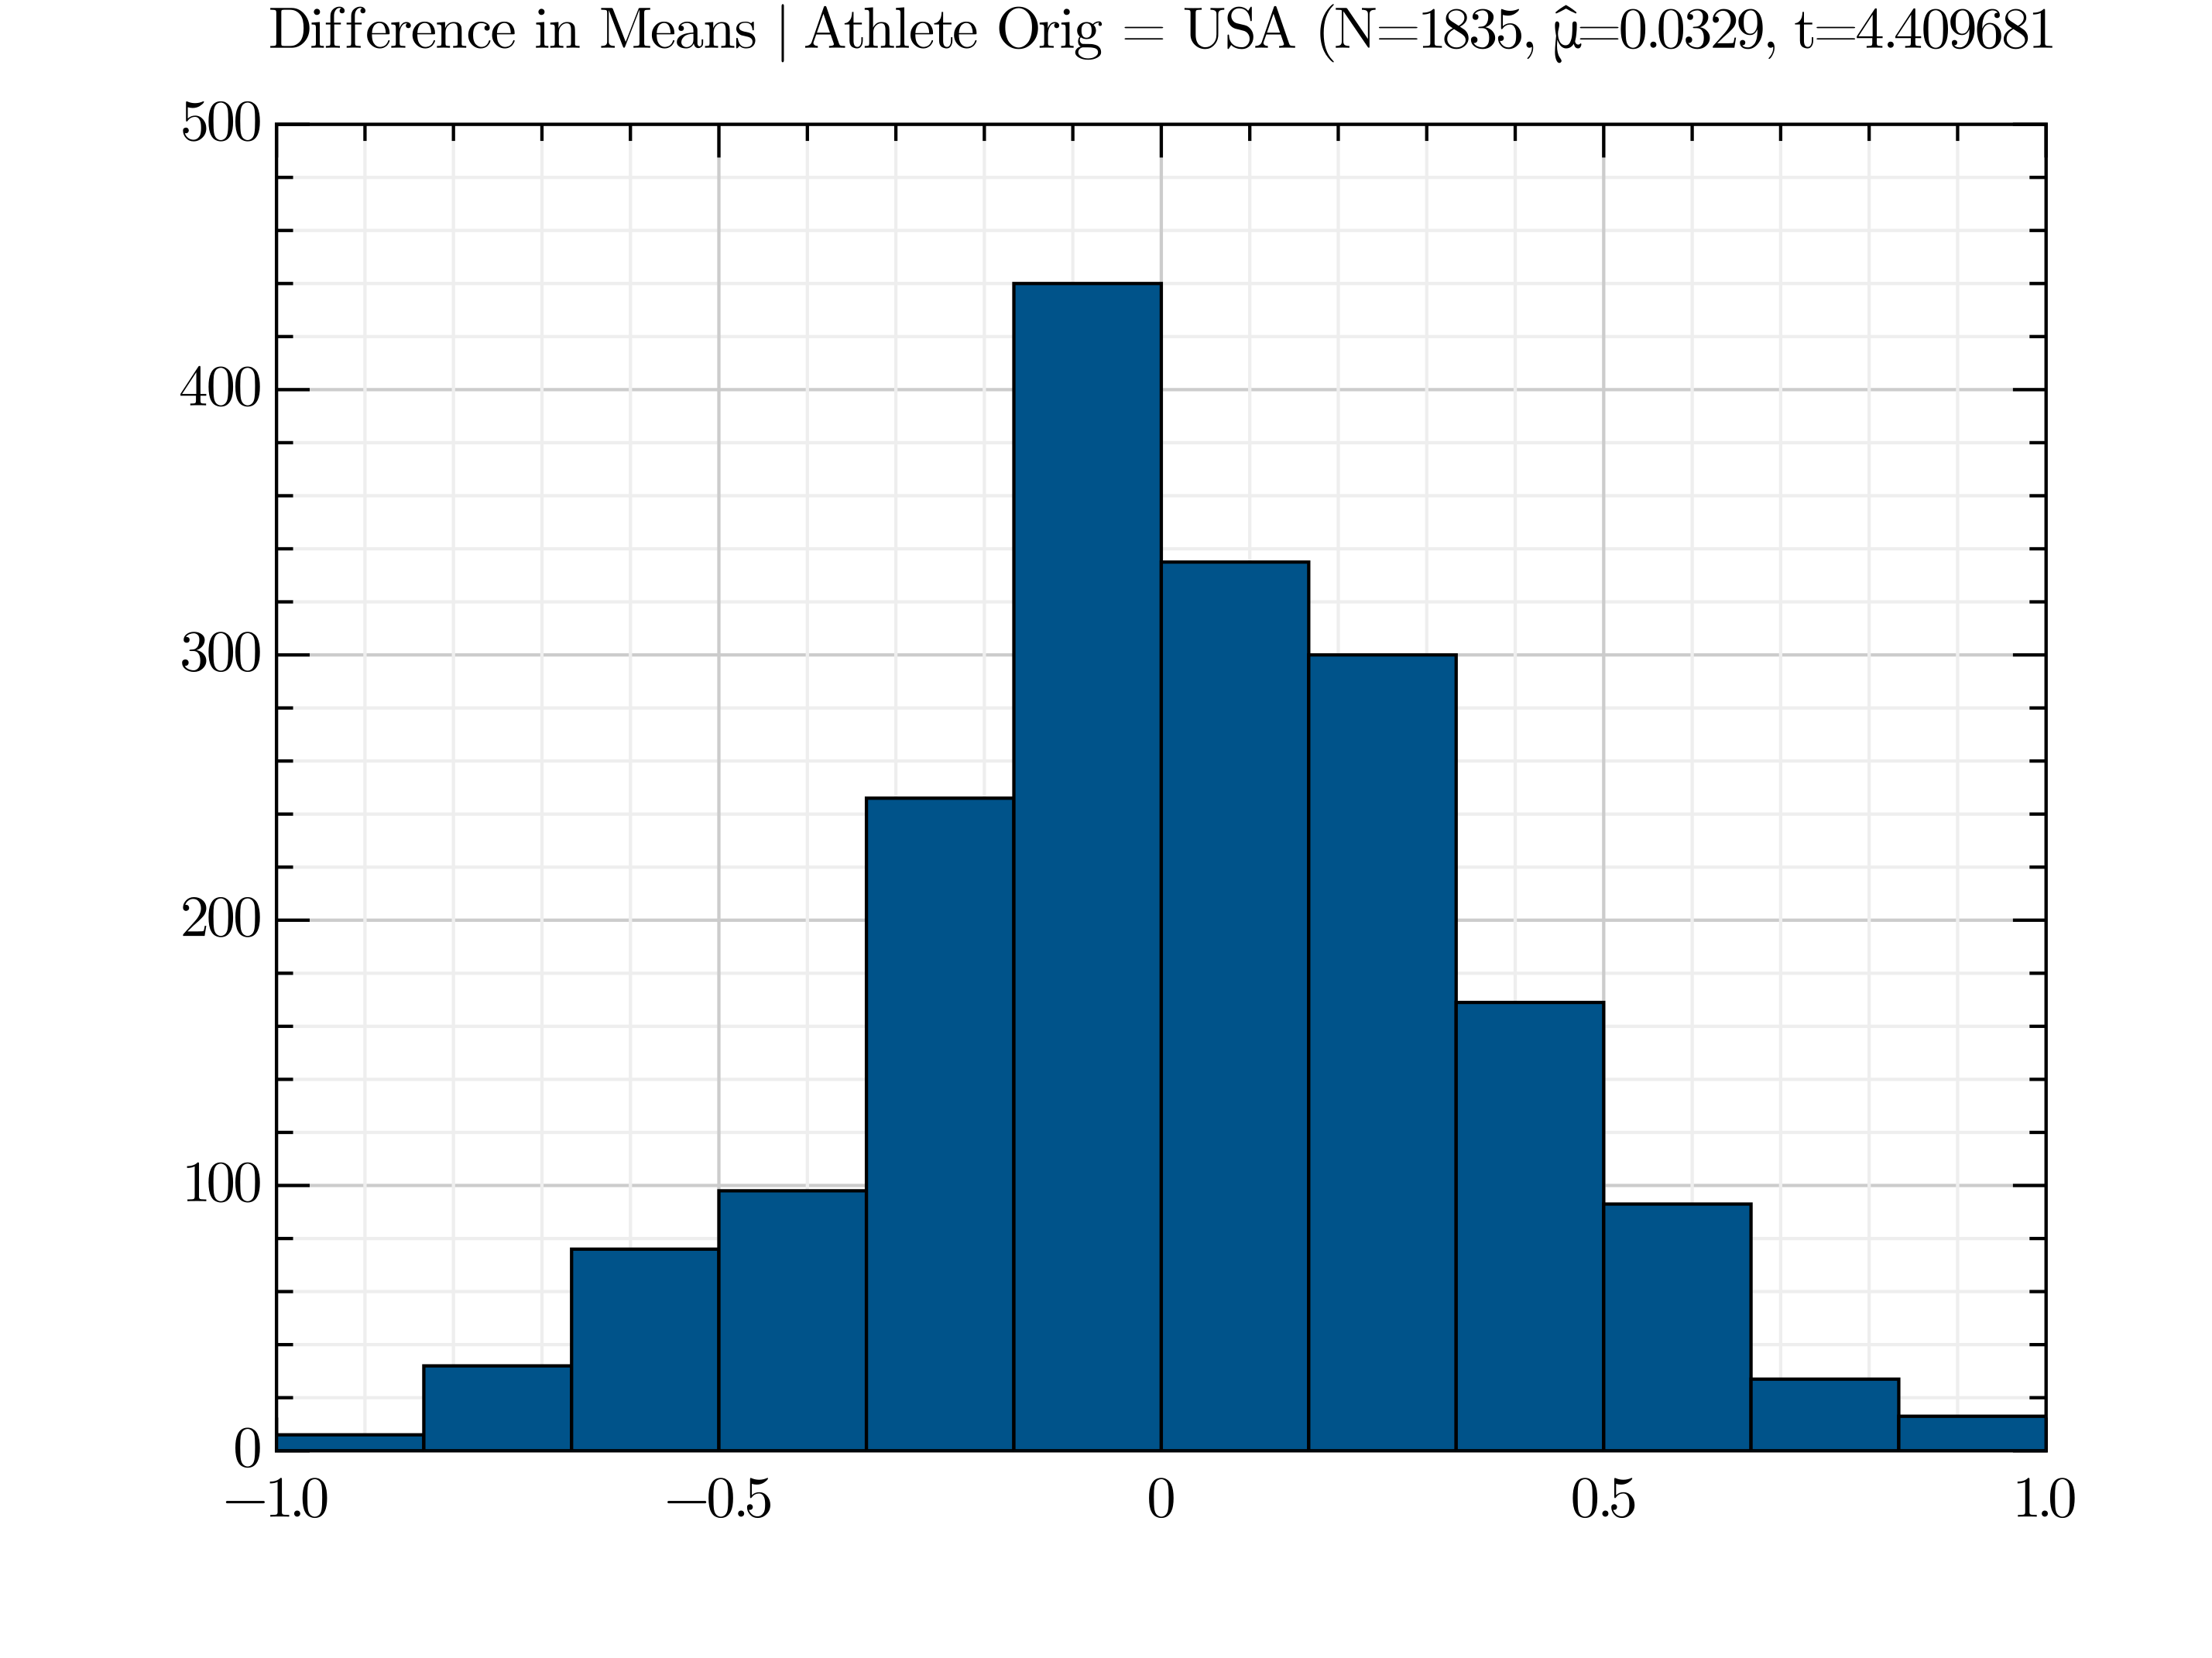
\includegraphics[width=8cm]{./src/visuals/DistOfDiffInMeansForUSA.png}
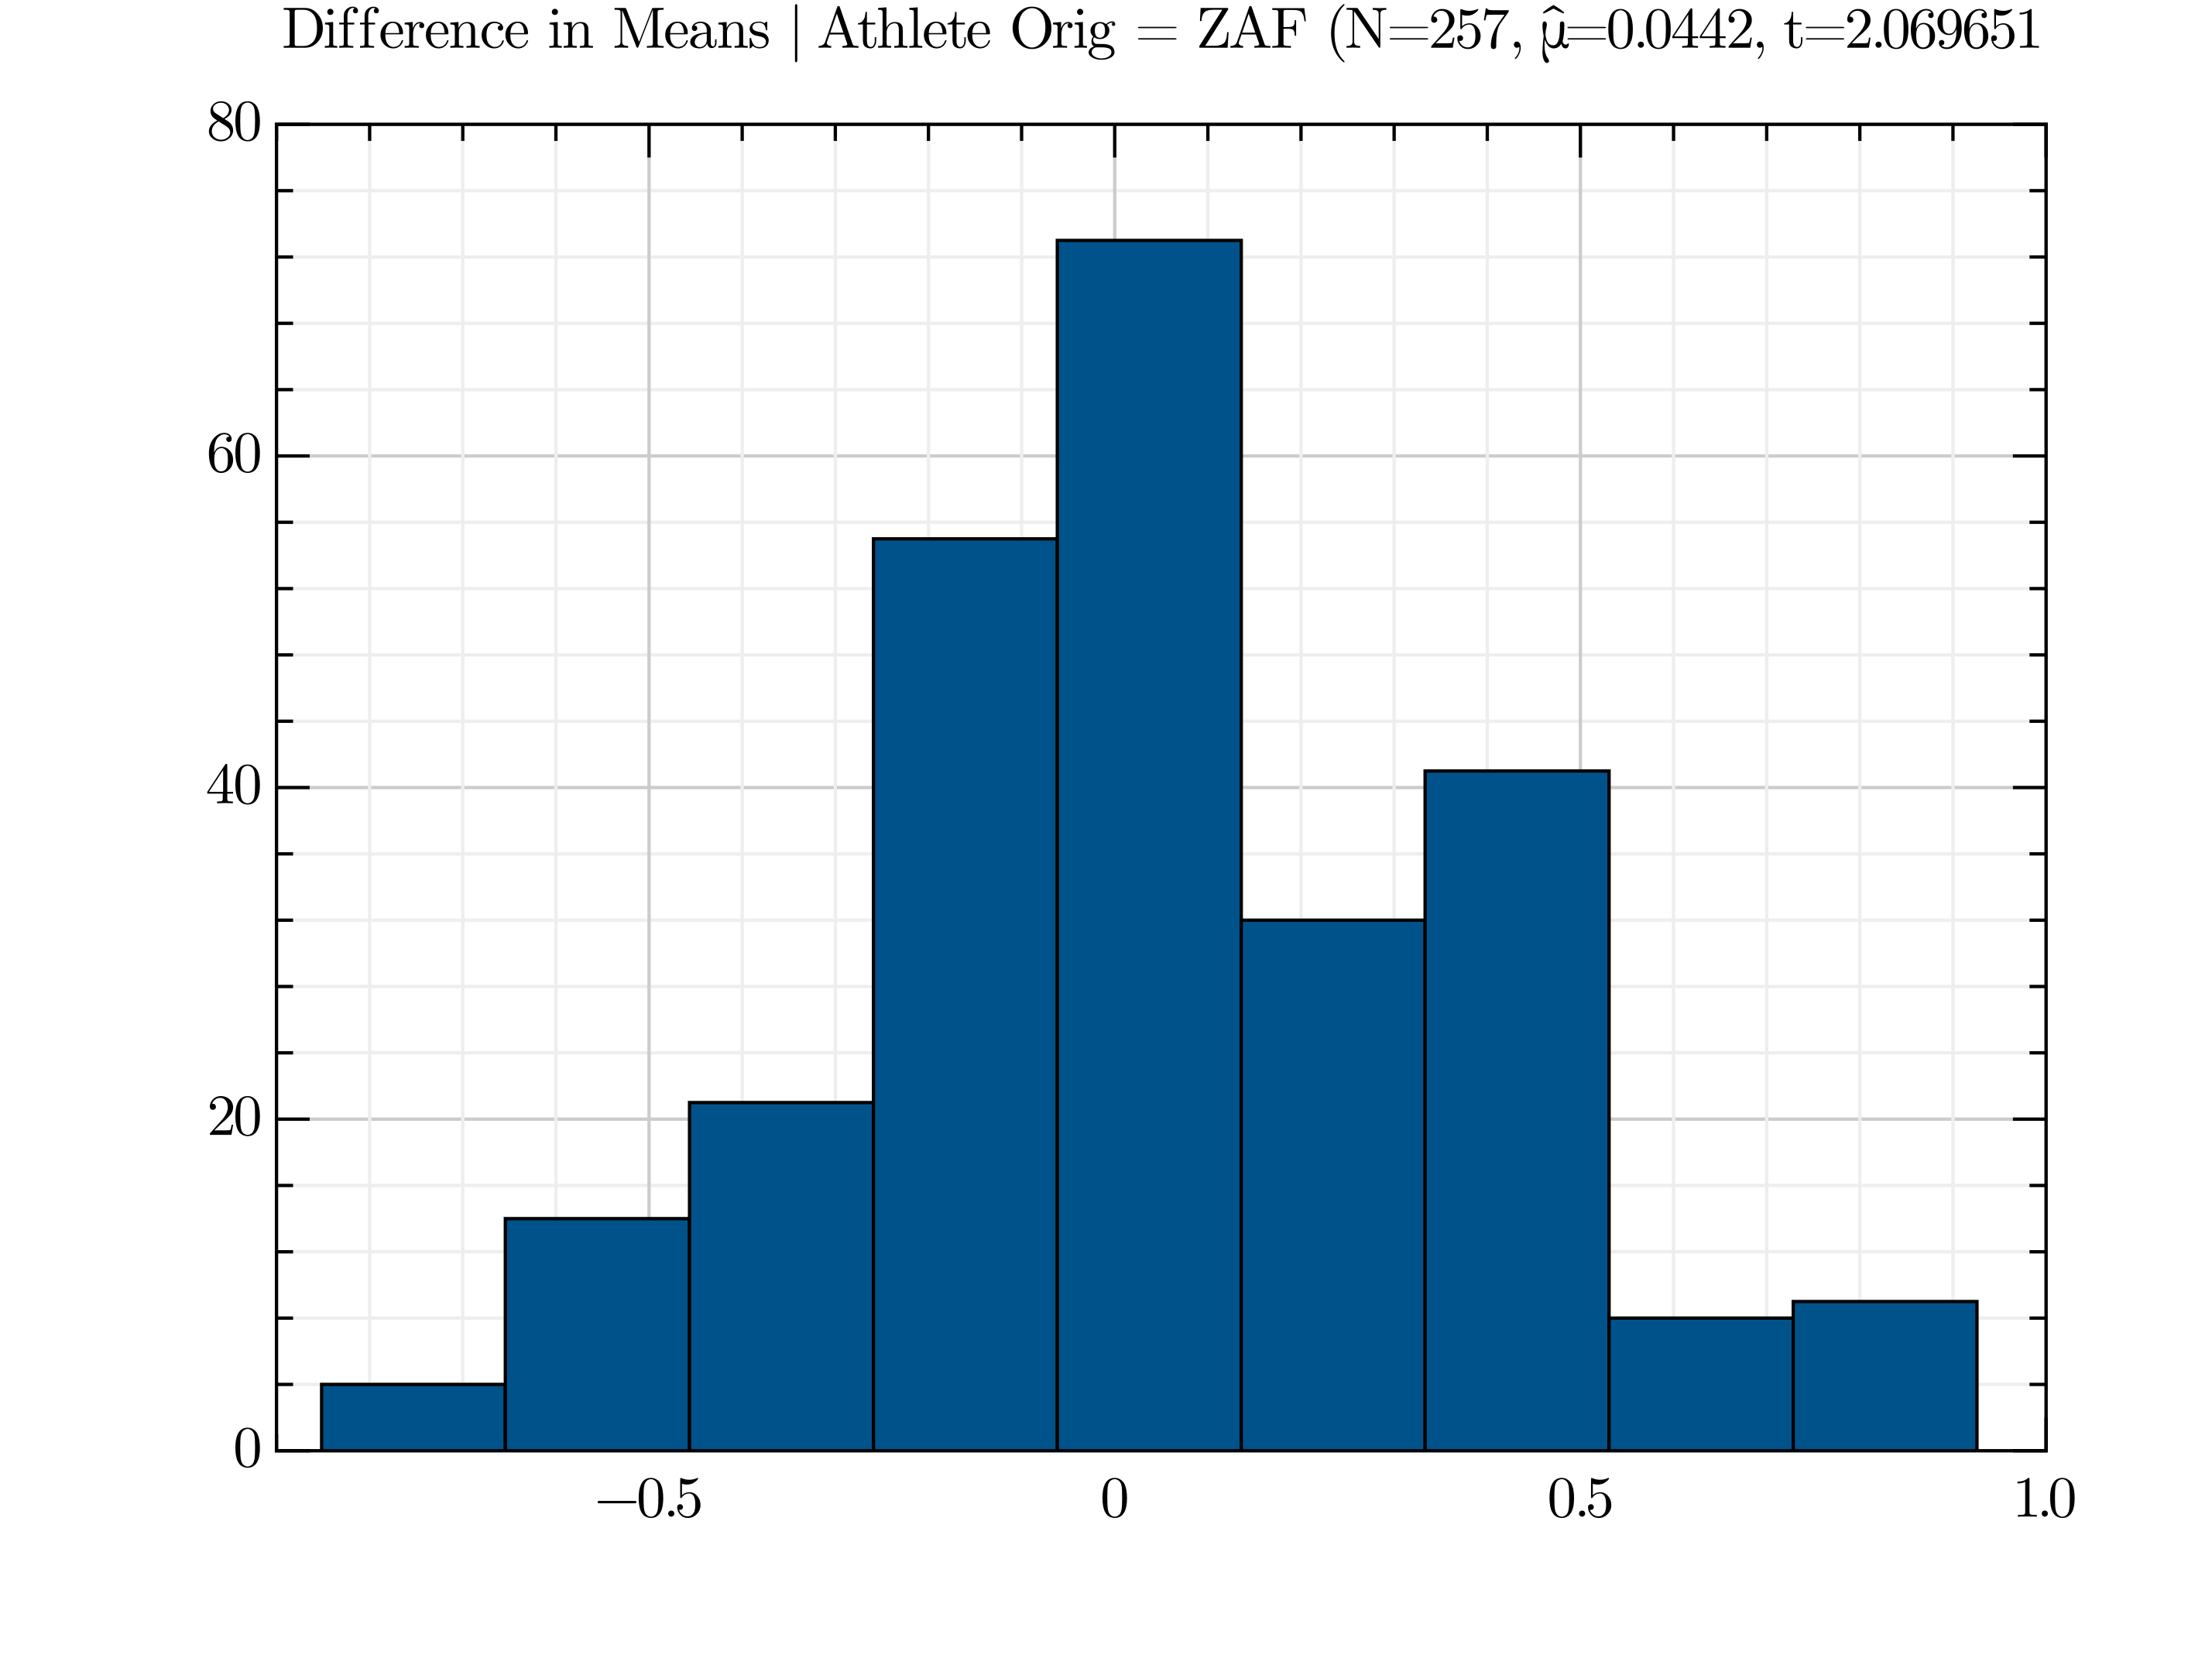
\includegraphics[width=8cm]{./src/visuals/DistOfDiffInMeansForZAF.png}

The difference of mean(DiffInMeans) is significant. However, the distribution of the differences in means is certainly less compelling. 

And we find that differences in means between Matching and Non-matching judges, conditional on a Nationality is significant for AUS, BRA, FRA, USA, ZAF. Though we will use the term "matching judge(s)" throughout the paper, it is important to keep in mind that it is the Athlete's origin which determines whether a judge is a "matching judge" or a "non-matching judge".


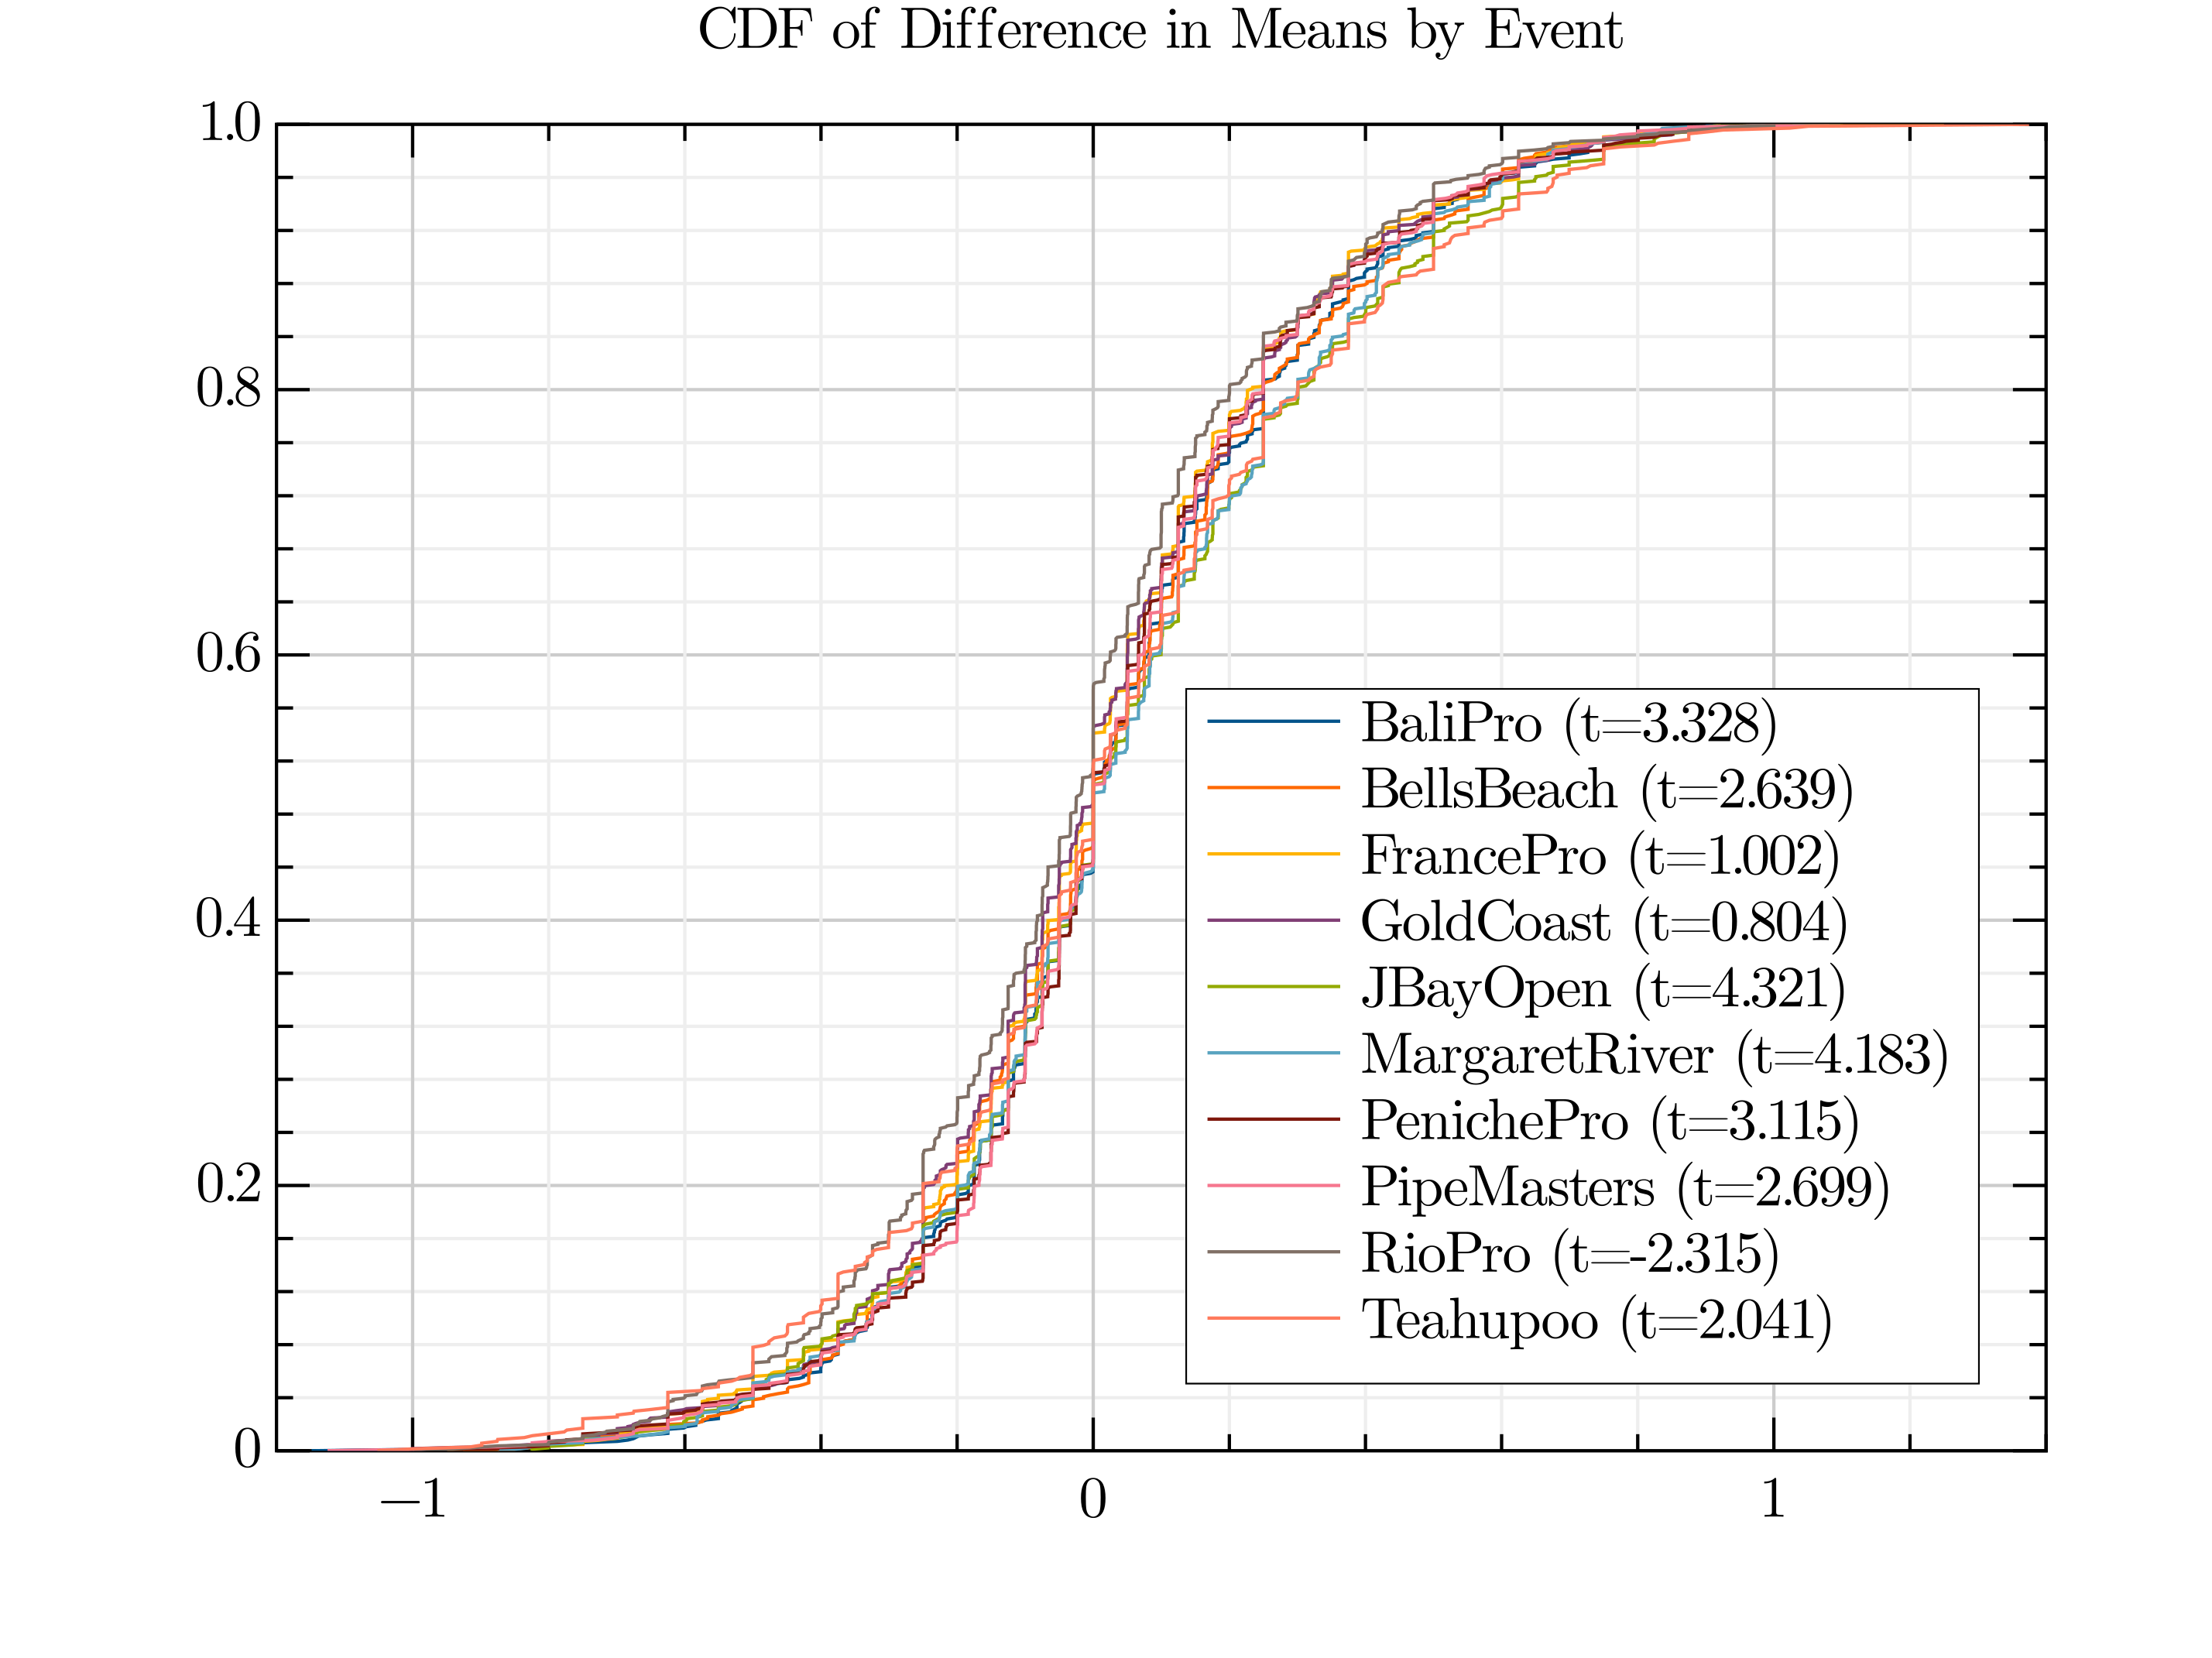
\includegraphics[width=8cm]{./src/visuals/DiffInMeansCDFbyevent.png}
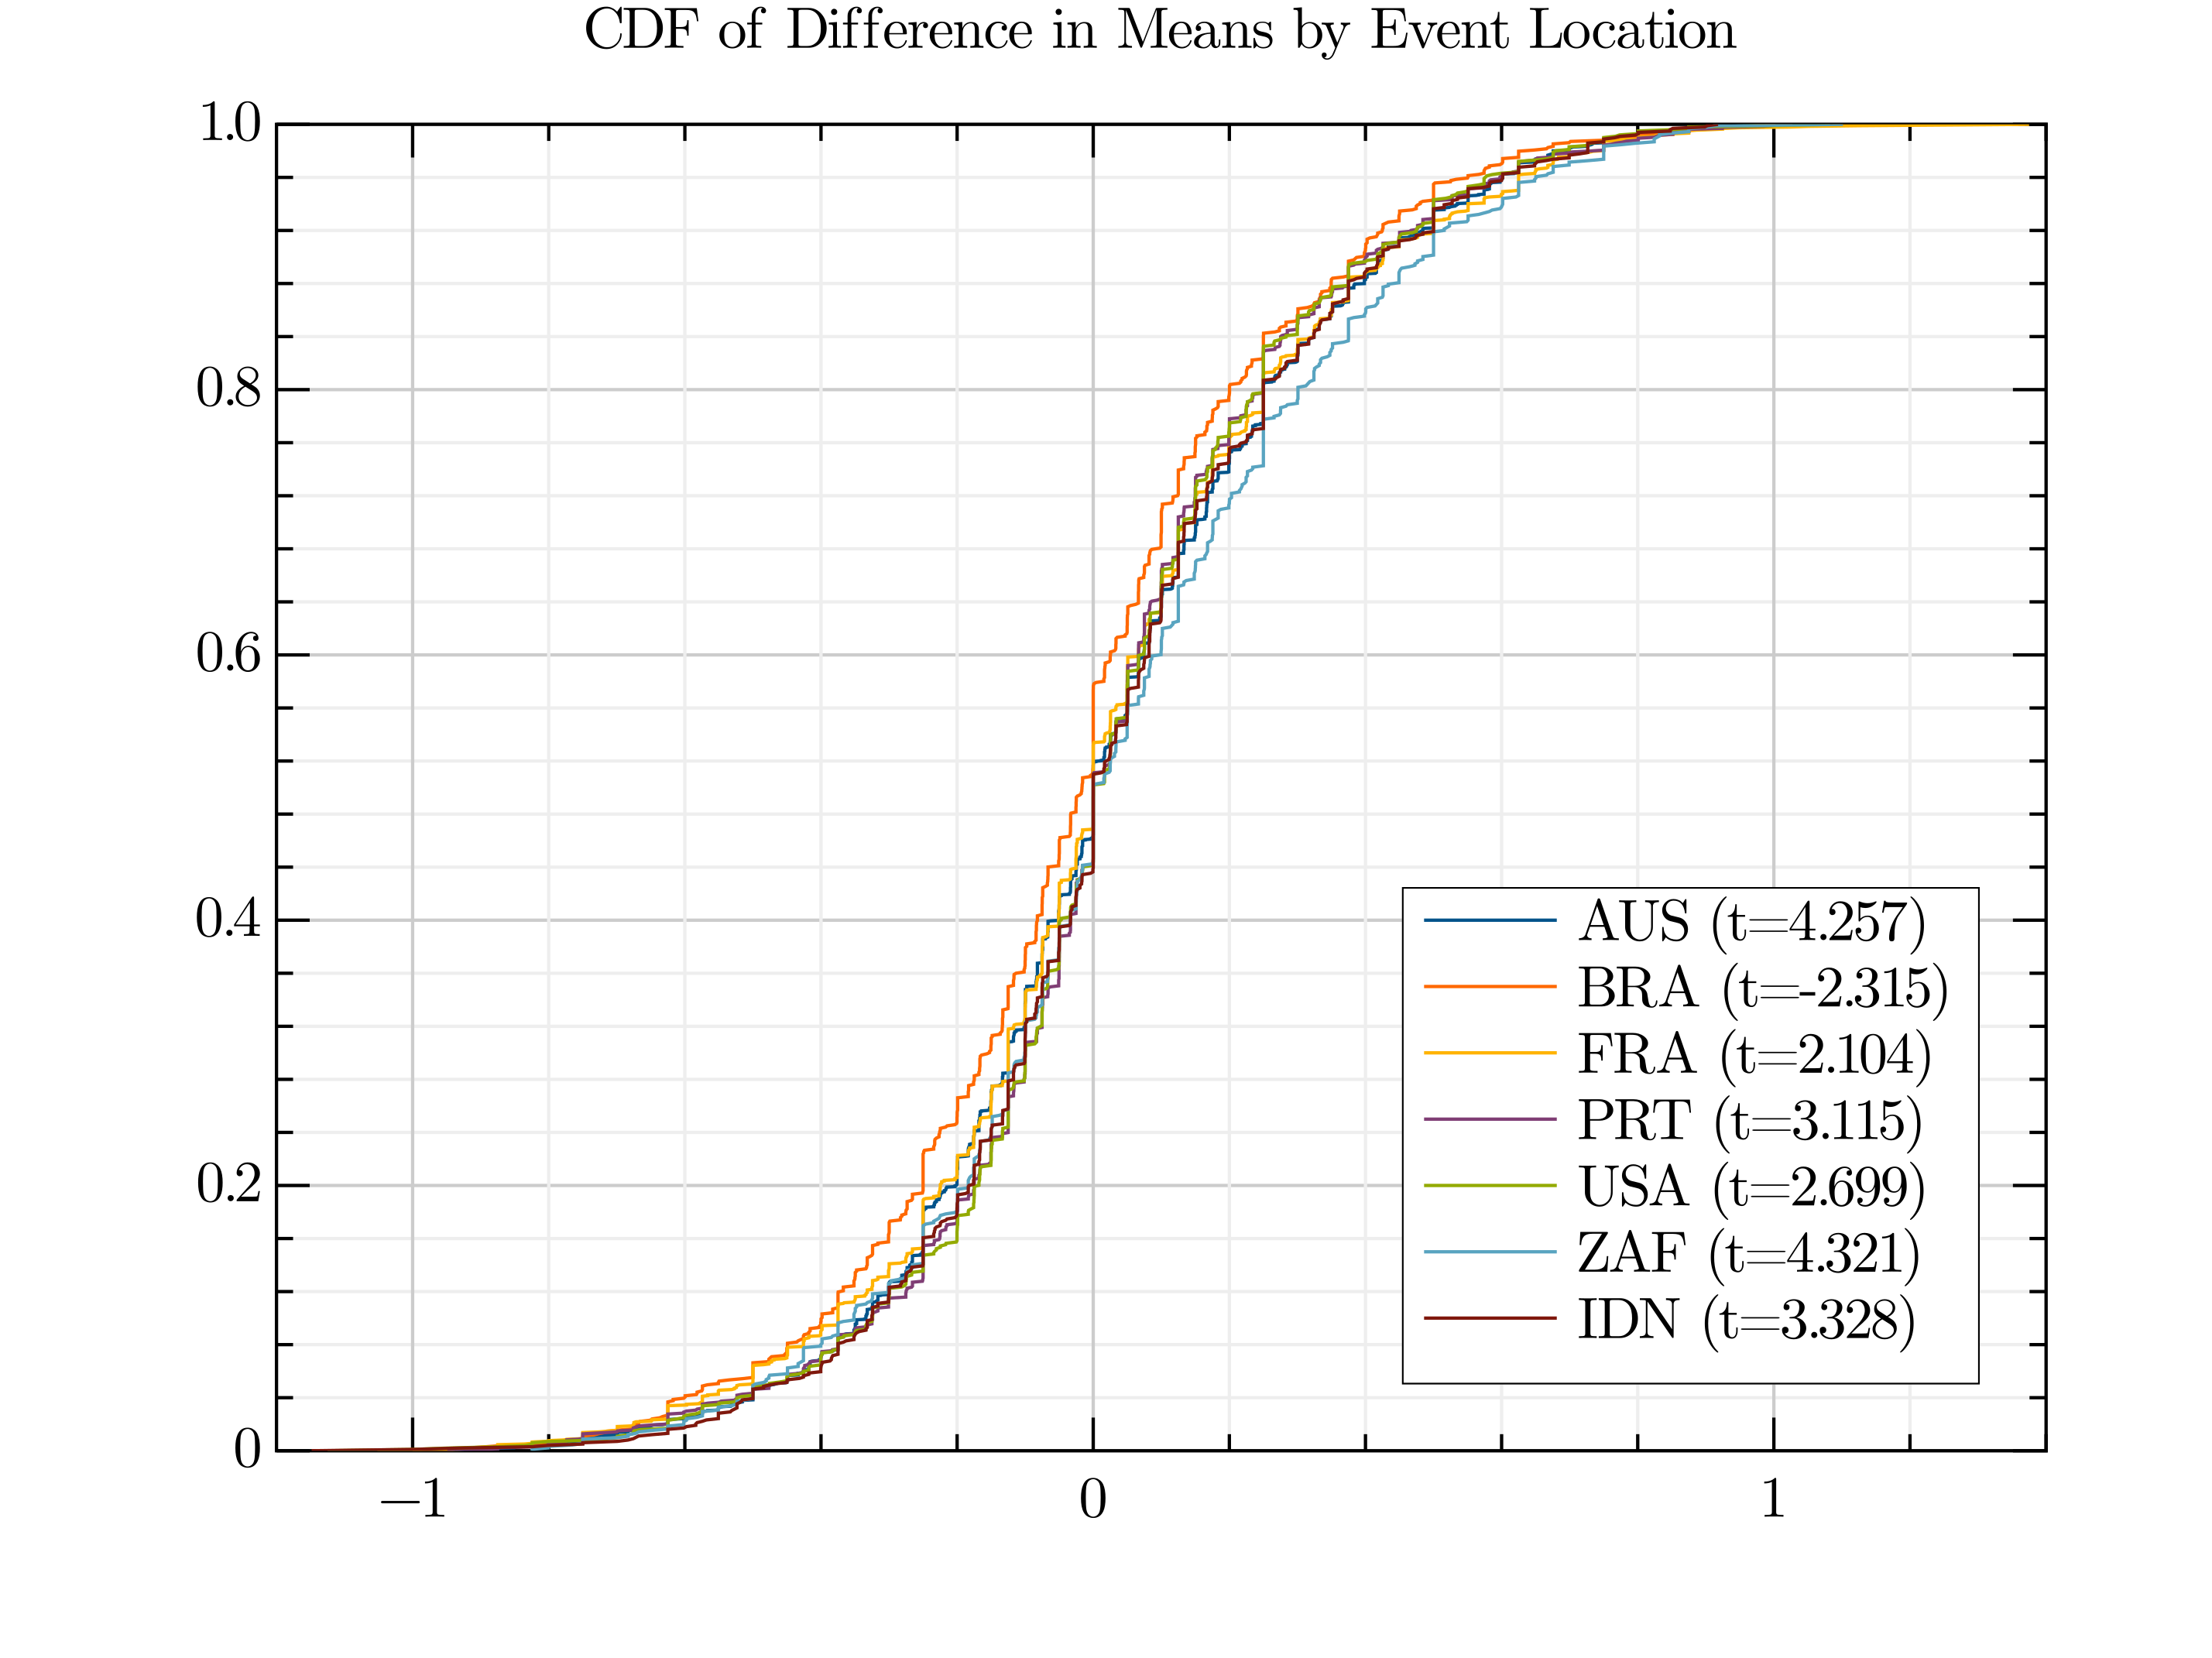
\includegraphics[width=8cm]{./src/visuals/DiffInMeansCDFbyeventOrig.png}
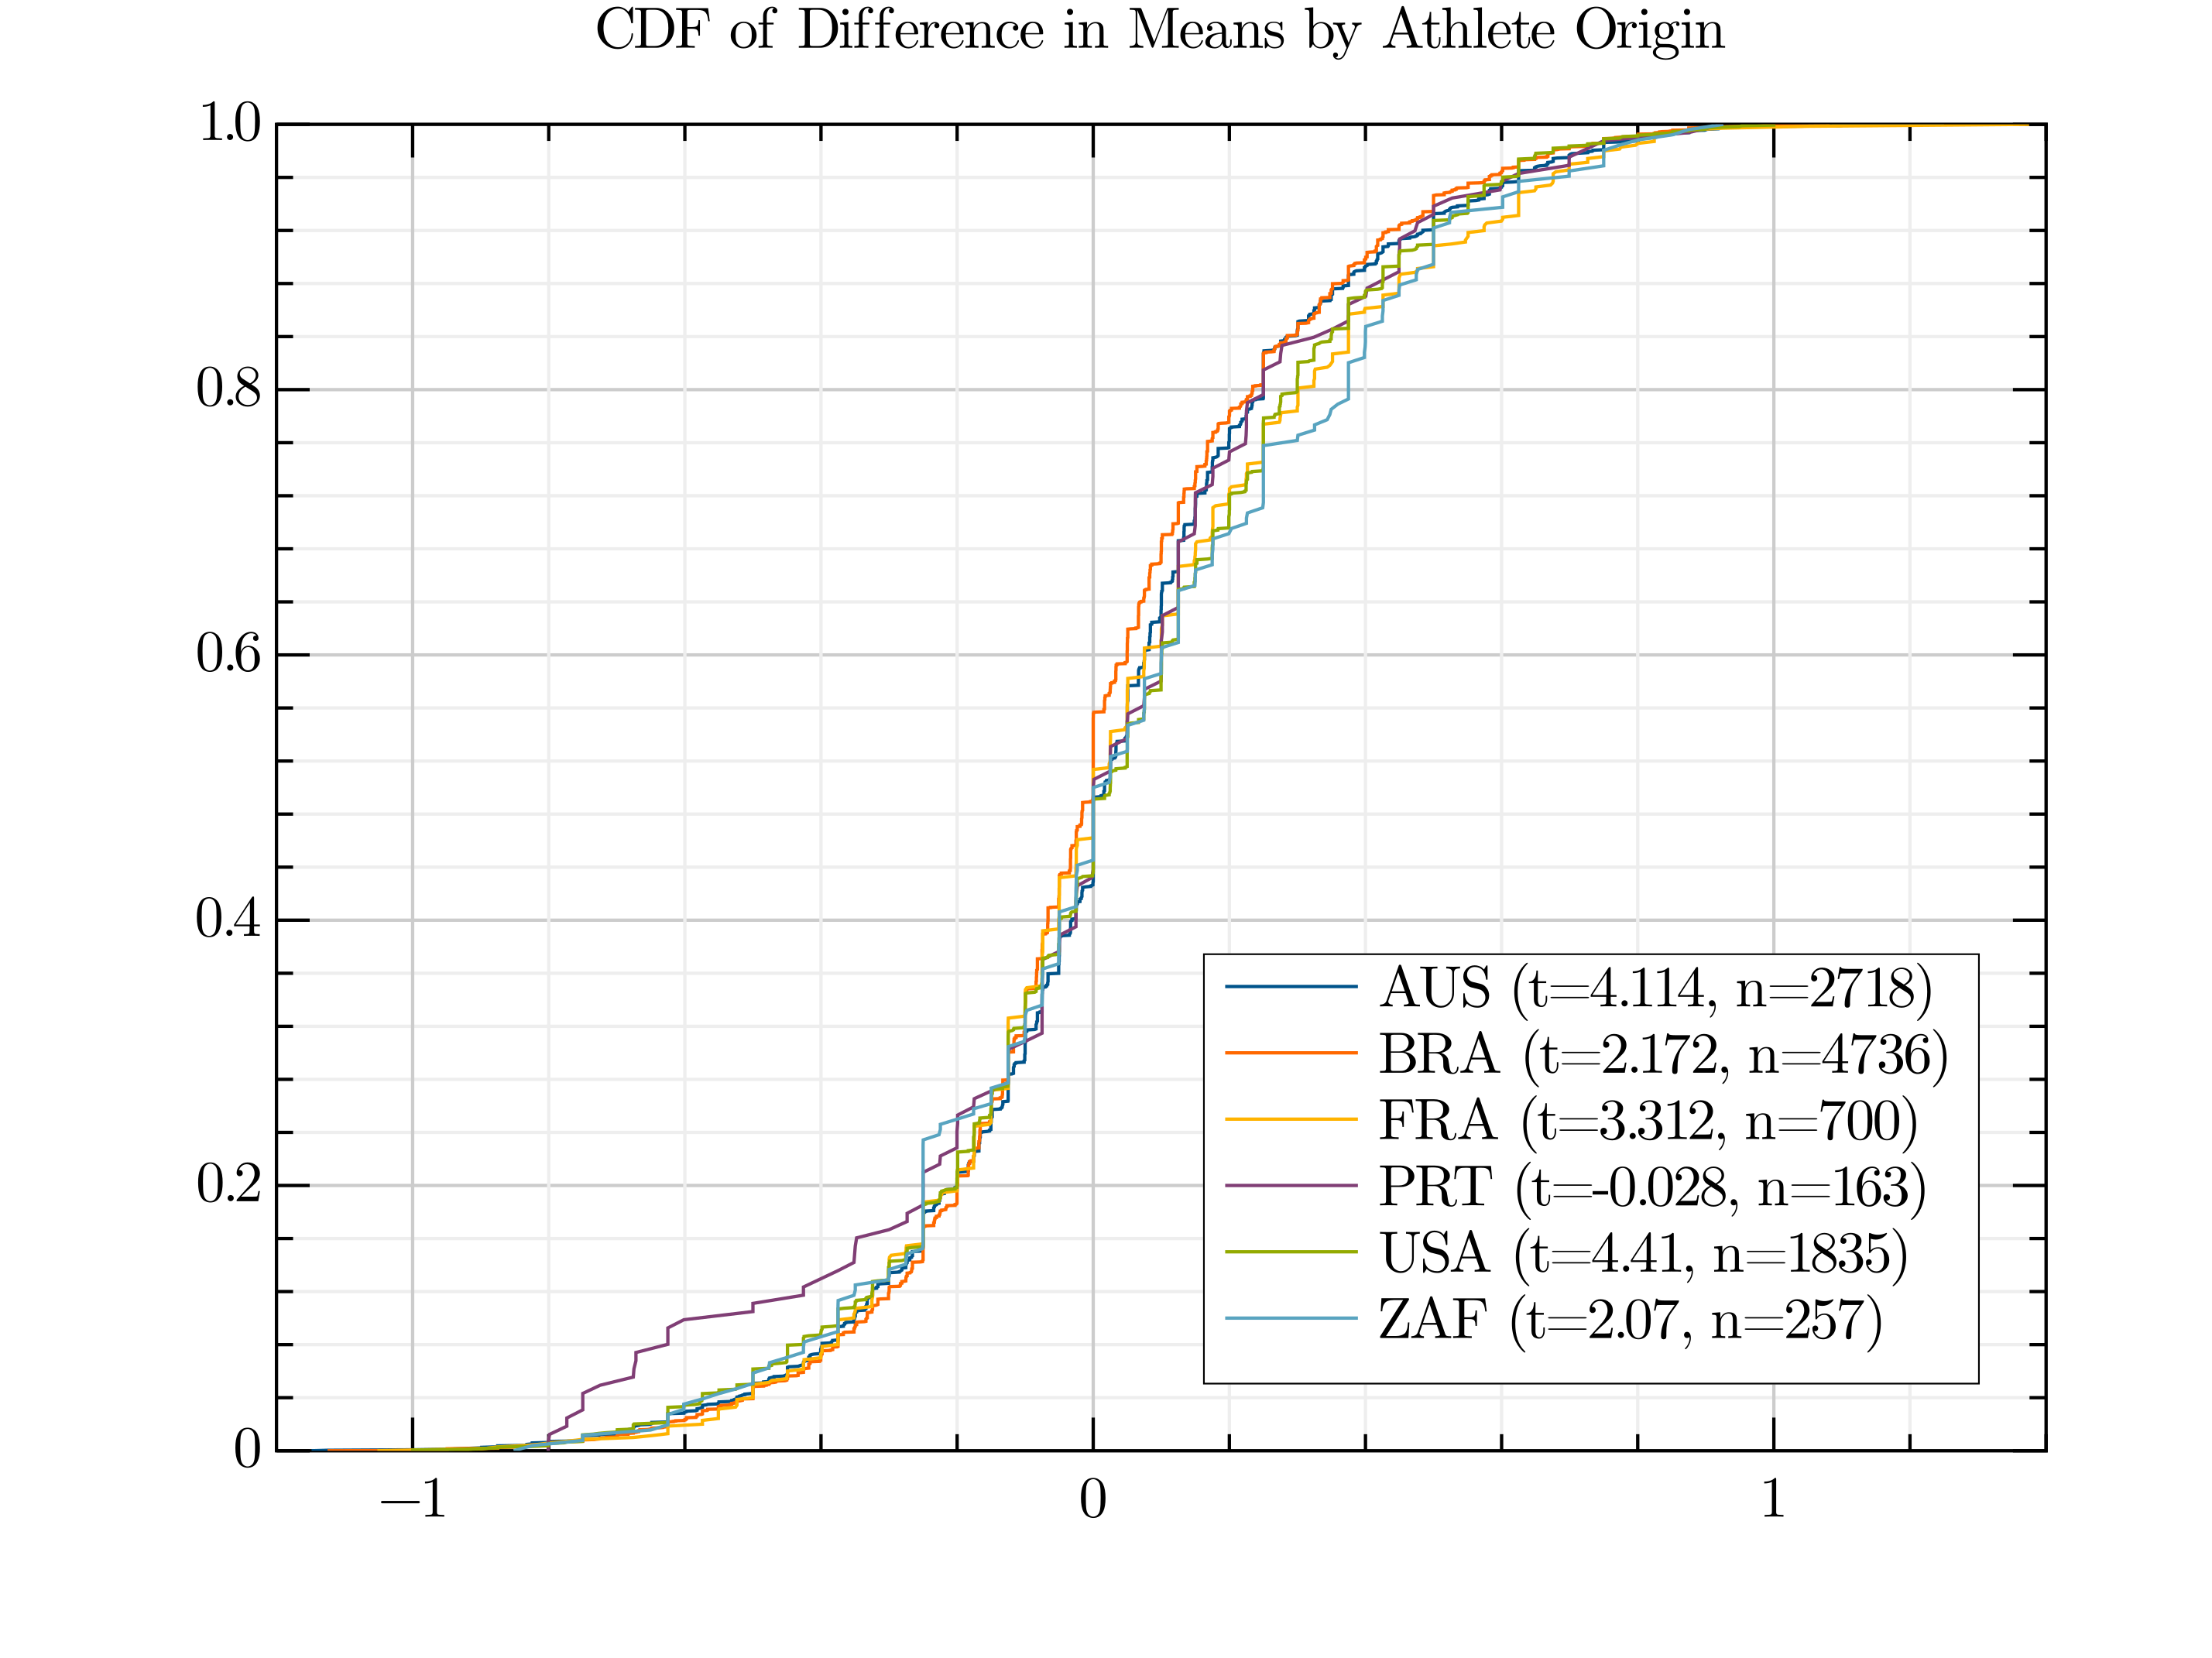
\includegraphics[width=8cm]{./src/visuals/DiffInMeansCDFbyathOrig.png}

\section{The Judging Panel}
Any given judging panel is comprised of 5 judges, we will denote this set of distinct humans by $J:=\{j_1,j_2,j_3,j_4,j_5\}$. Each judge has a nationality, $c_i \in \{AUS,BRA,ESP,FRA,PRT,USA,ZAF\}$. When a surfer attempts to ride a wave, each judge writes down some score $s_i \in \{0.1,0.2,\dots,9.9,10.0\}$. So for any given wave we observe 5 pairs $[(c_1,s_1),(c_2,s_2),(c_3,s_3),(c_4,s_4),(c_5,s_5)]$. Sometimes two judges have the same nationality and write down the same score. 

We'd like to introduce two examples/instances of a heat that we will use throughout the paper. They are the first two heats of the 2018 season; in particular, Heat 1 and 2 of Round 1 of first event of 2018 called "Quiksilver Pro Gold Coast".

In Round 1 Heat 1 of the "Gold Coast" event, located in Australia, the panel consists of 5 judges. Their nationalities are $[AUS,BRA,ESP, USA,ZAF]$. Caio Ibelli, a Brazilian surfer, takes the first wave of the heat and the panel gives the following scores for his efforts: $ [(AUS,0.5), (BRA,0.3),(ESP,0.5),(USA,0.5),(ZAF,0.3)]$. The scores are $[0.5,0.3,0.5,0.5,0.3]$, so the mean score is $1/5(0.5+0.3+0.5+0.5+0.3) = 0.42$, and the "WSL Score" is mean of the panel's scores with (one of) the highest and lowest score dropped, $1/3(0.3+0.5+0.5) = 0.4\bar{3}$, which is rounded to $0.43$. Below is the series of wave scores for the Round 1 Heat 1.

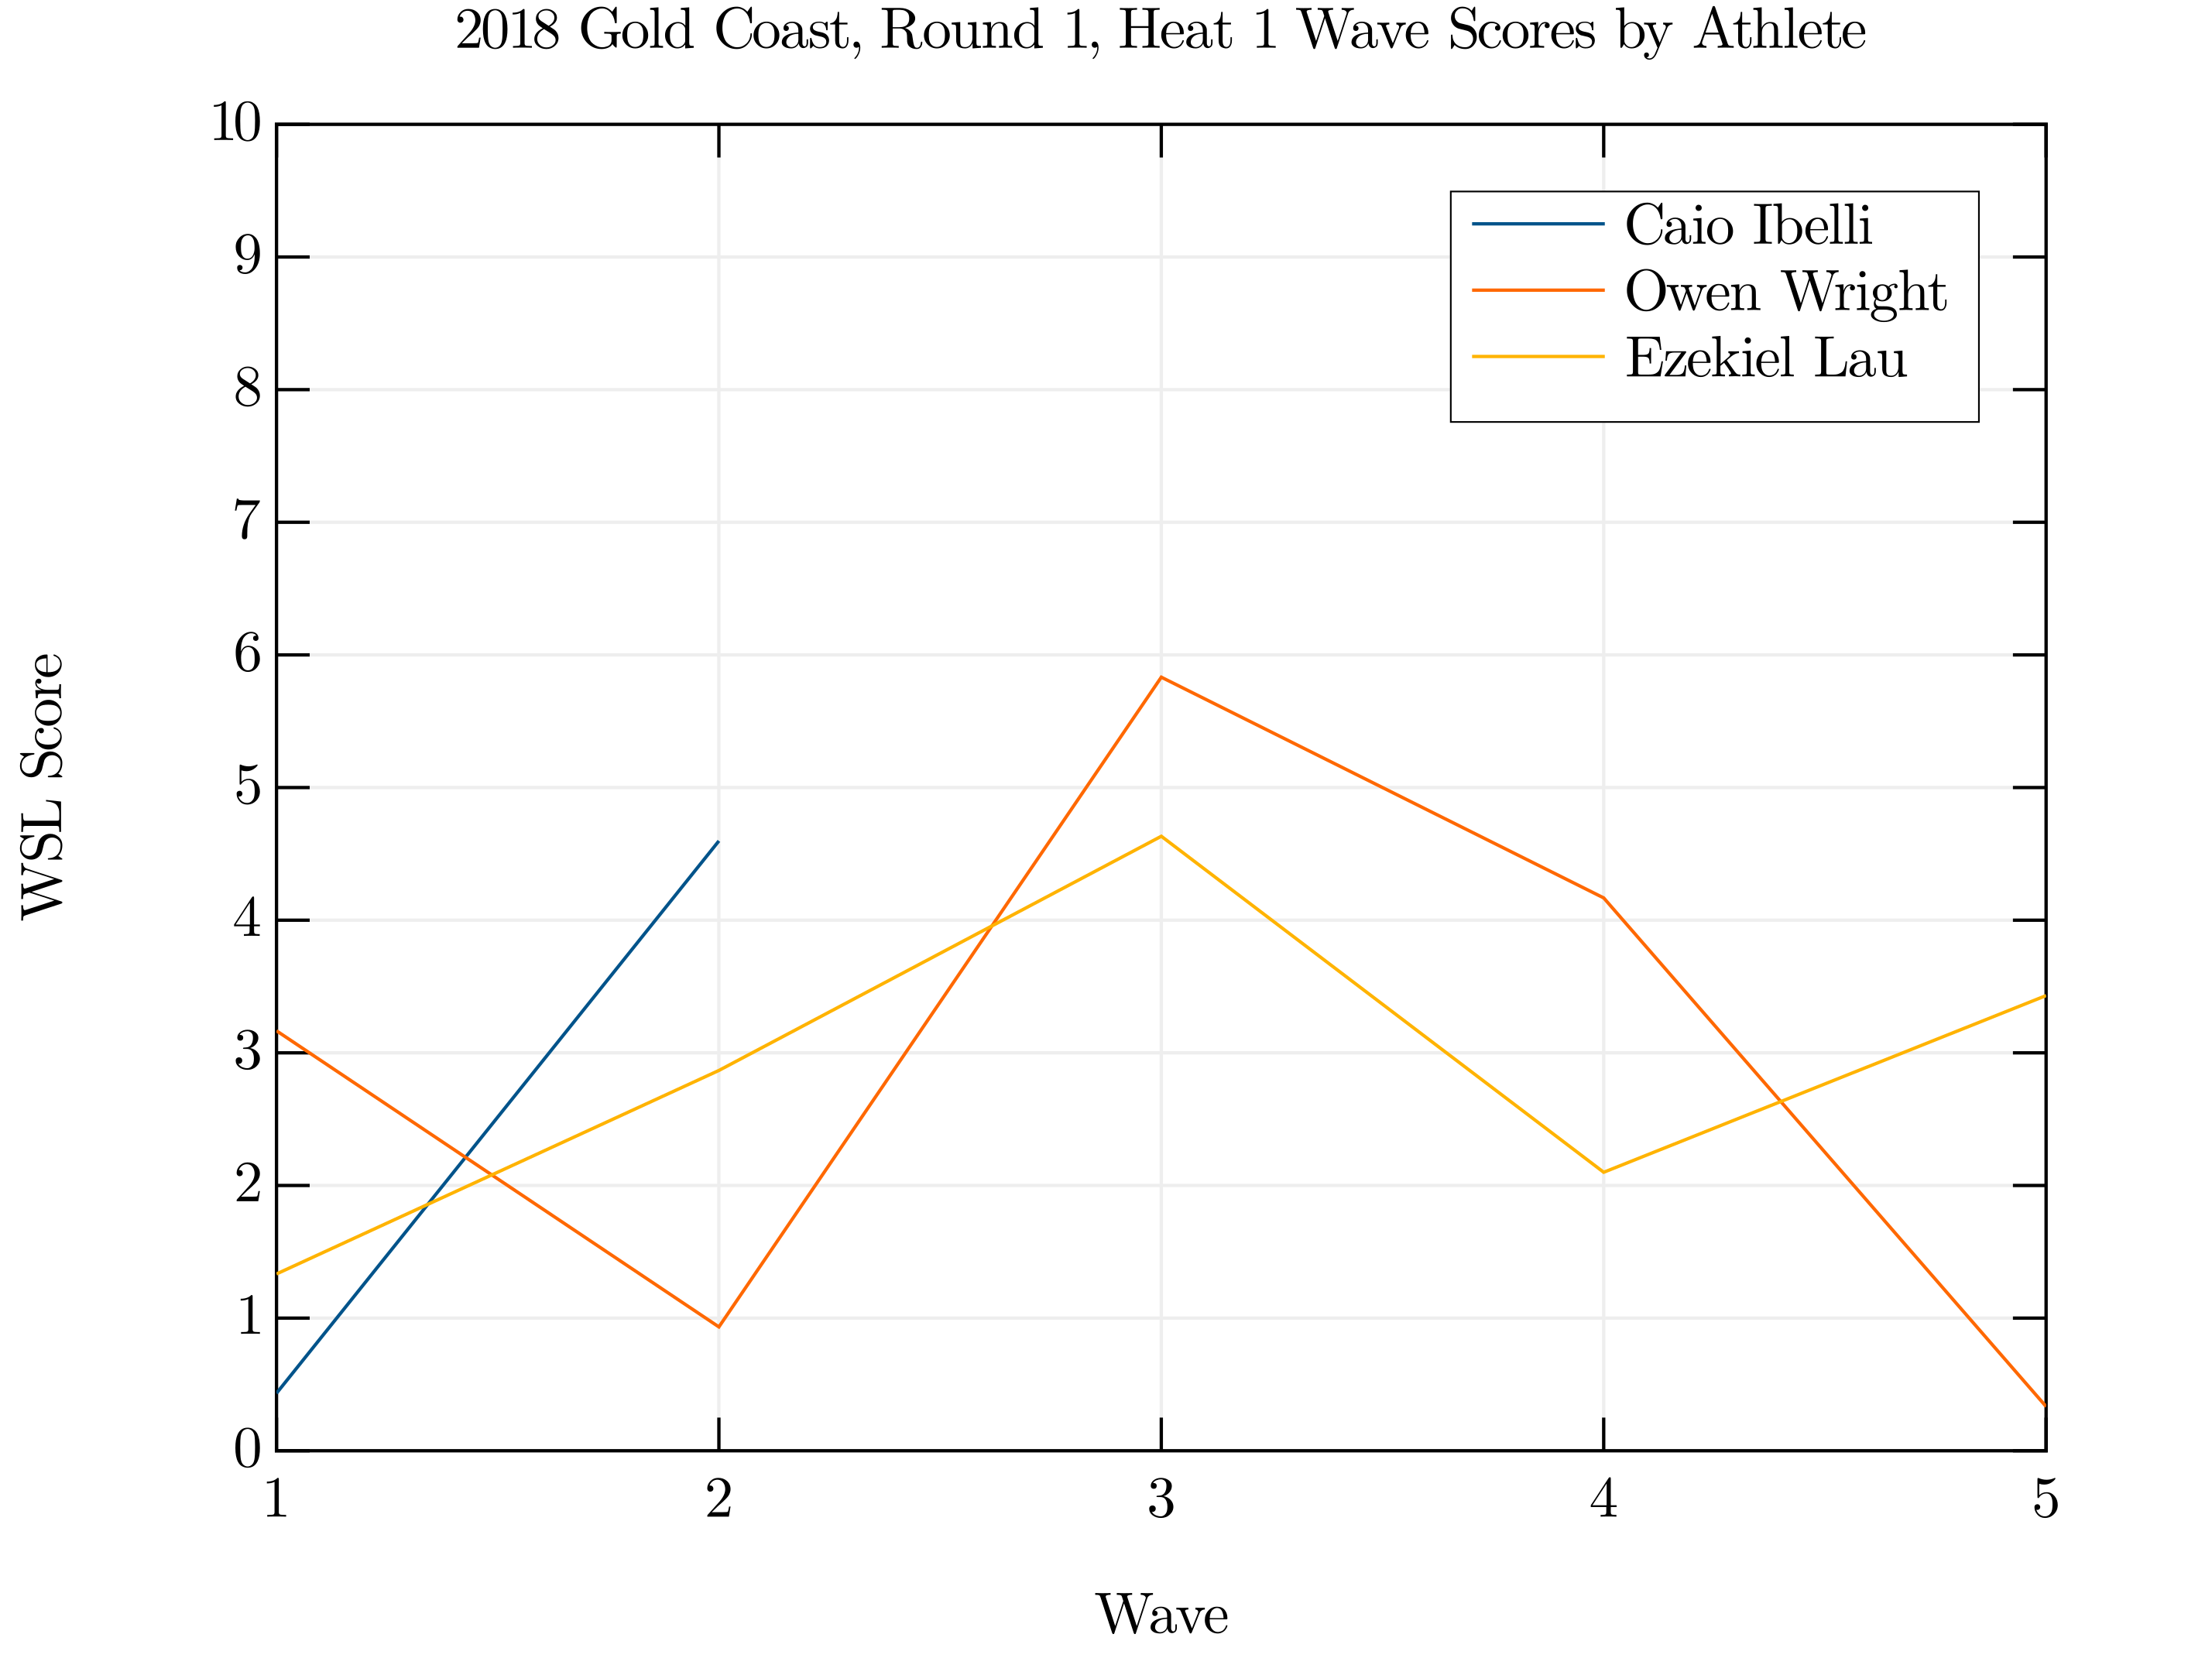
\includegraphics[width=6cm]{./src/visuals/2018GCR1/WaveScoresByAthH1.png}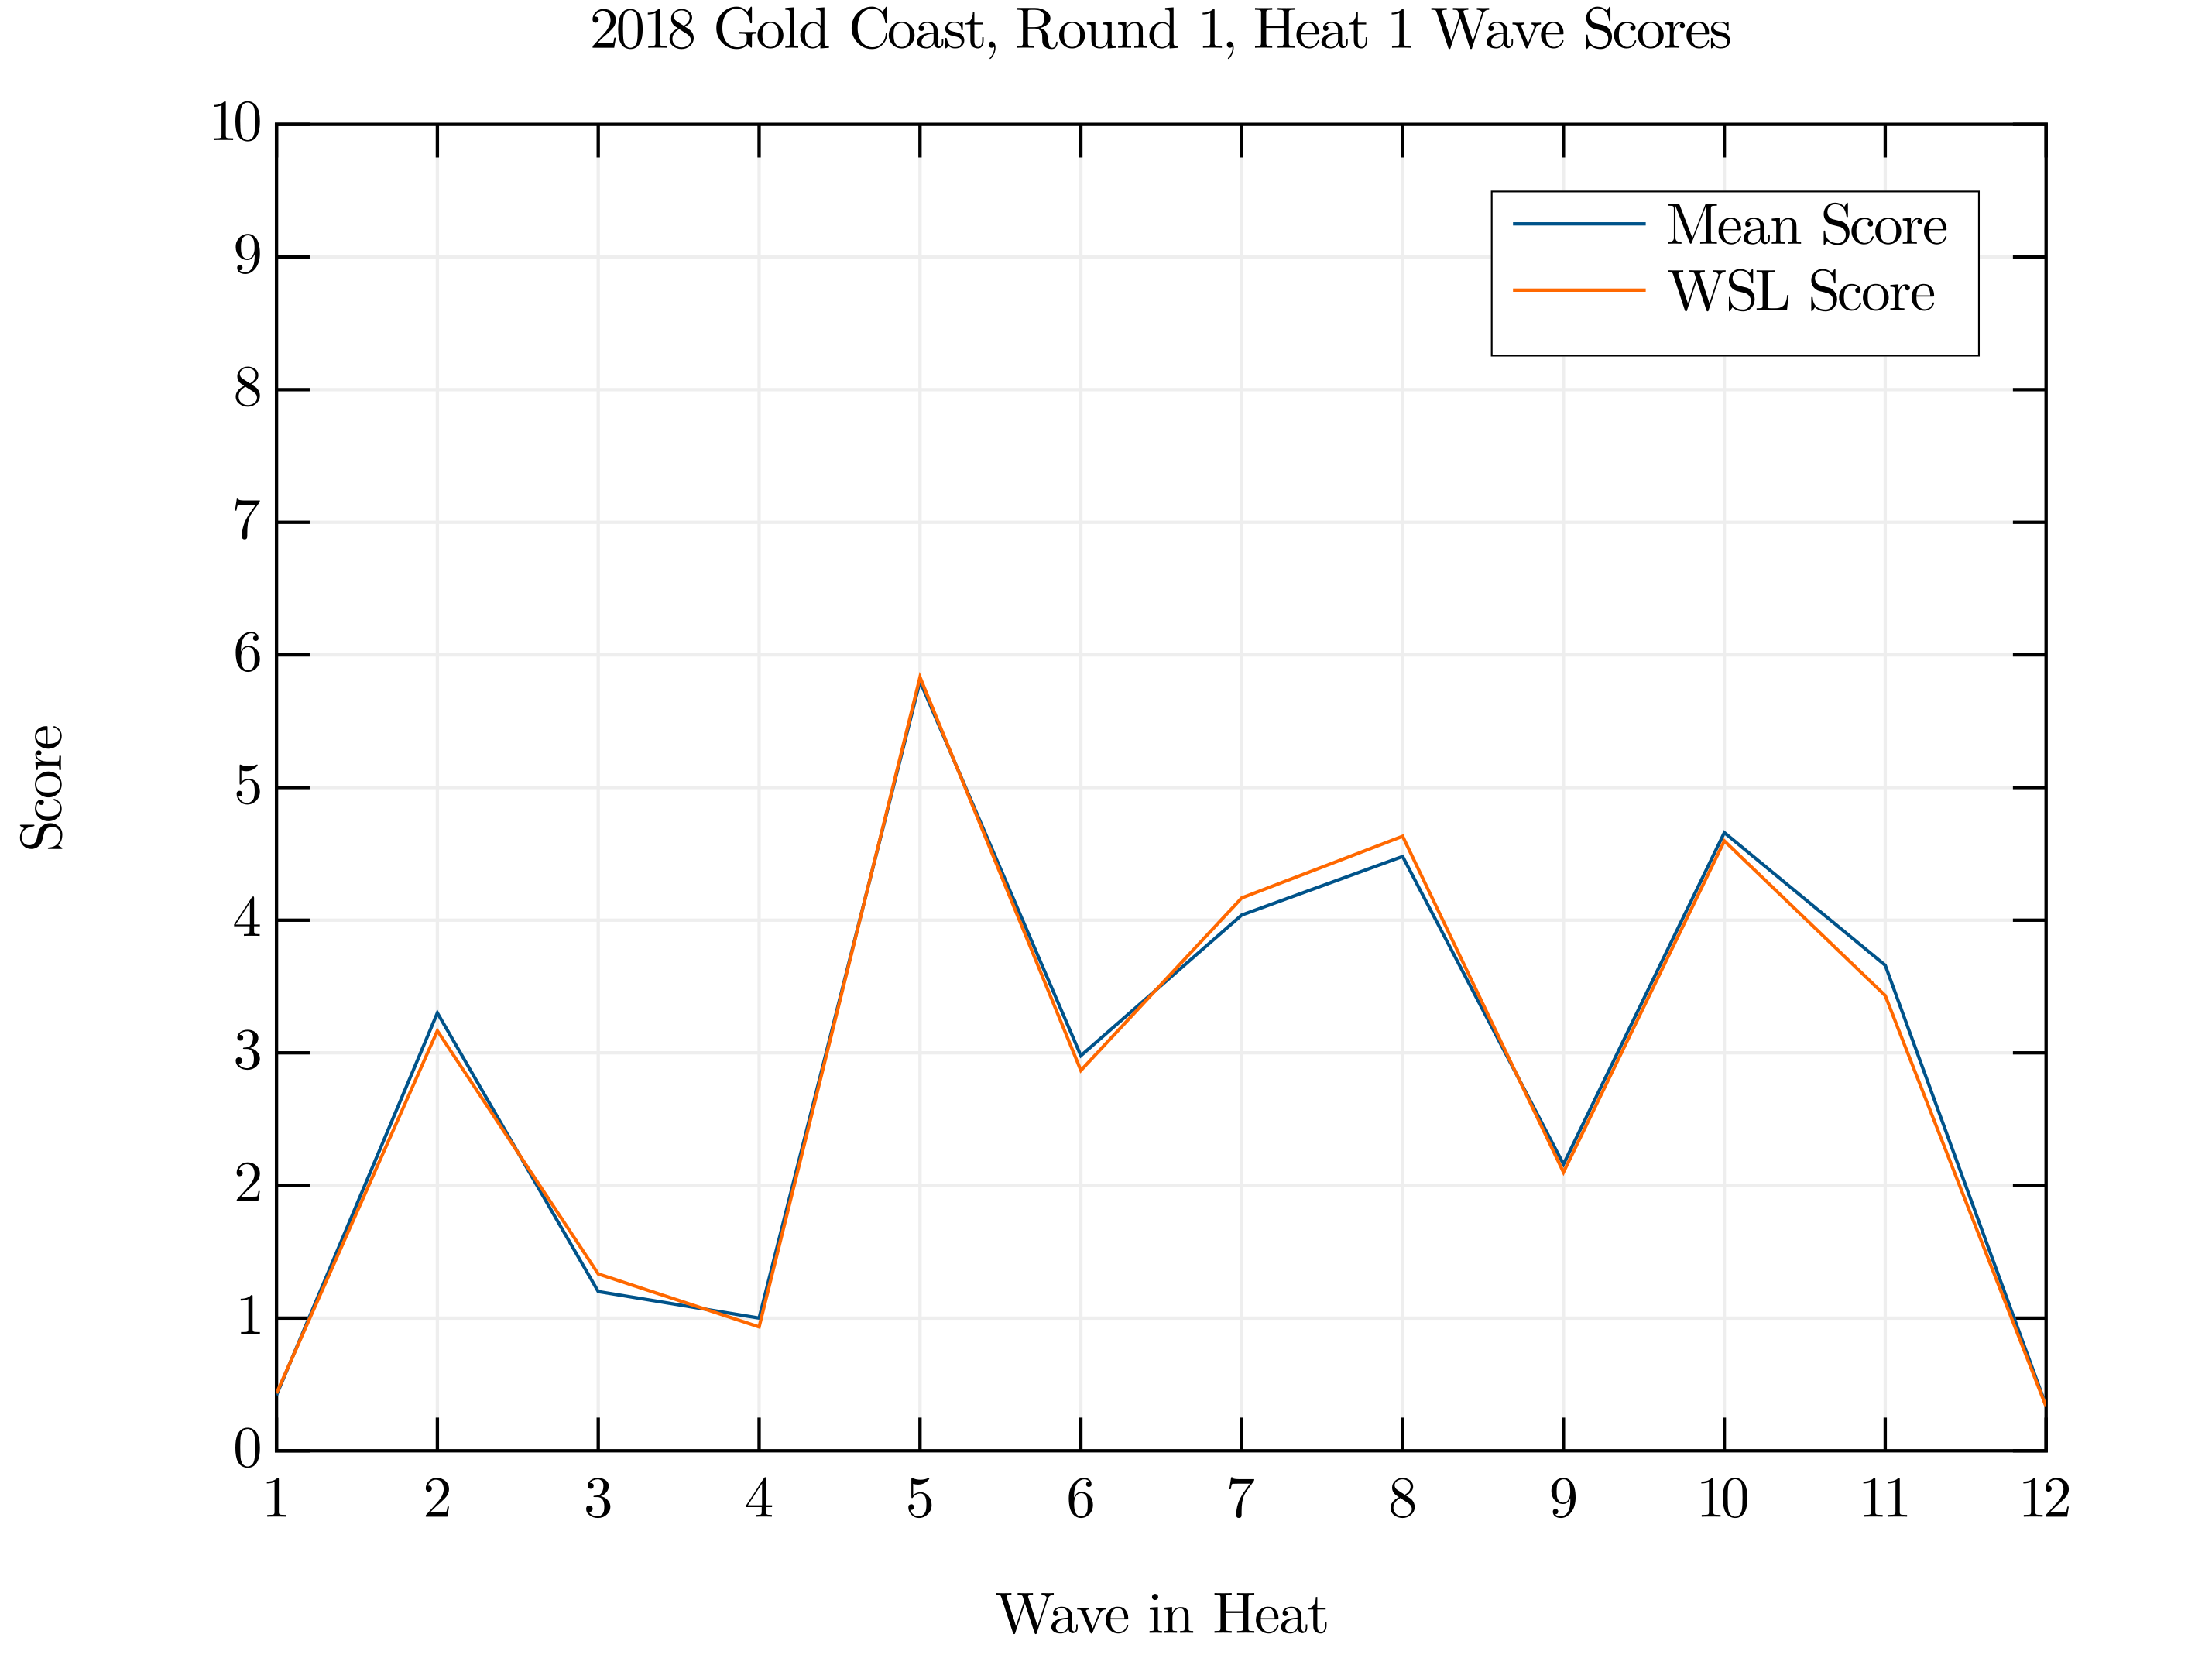
\includegraphics[width=6cm]{./src/visuals/2018GCR1/WaveScoresH1.png}


In Round 1 Heat 2 of the Gold Coast event, the panel consists of 5 judges, and their nationalities are $[AUS,AUS,BRA,BRA,USA]$. Michael Rodrigues rides the first wave of the heat and we observe the panel: $[(AUS,0.3),(AUS,0.3),(BRA,0.2),(BRA,0.5),(USA,0.3)]$. The mean score of this wave is 0.32, and the WSL score is 0.30.

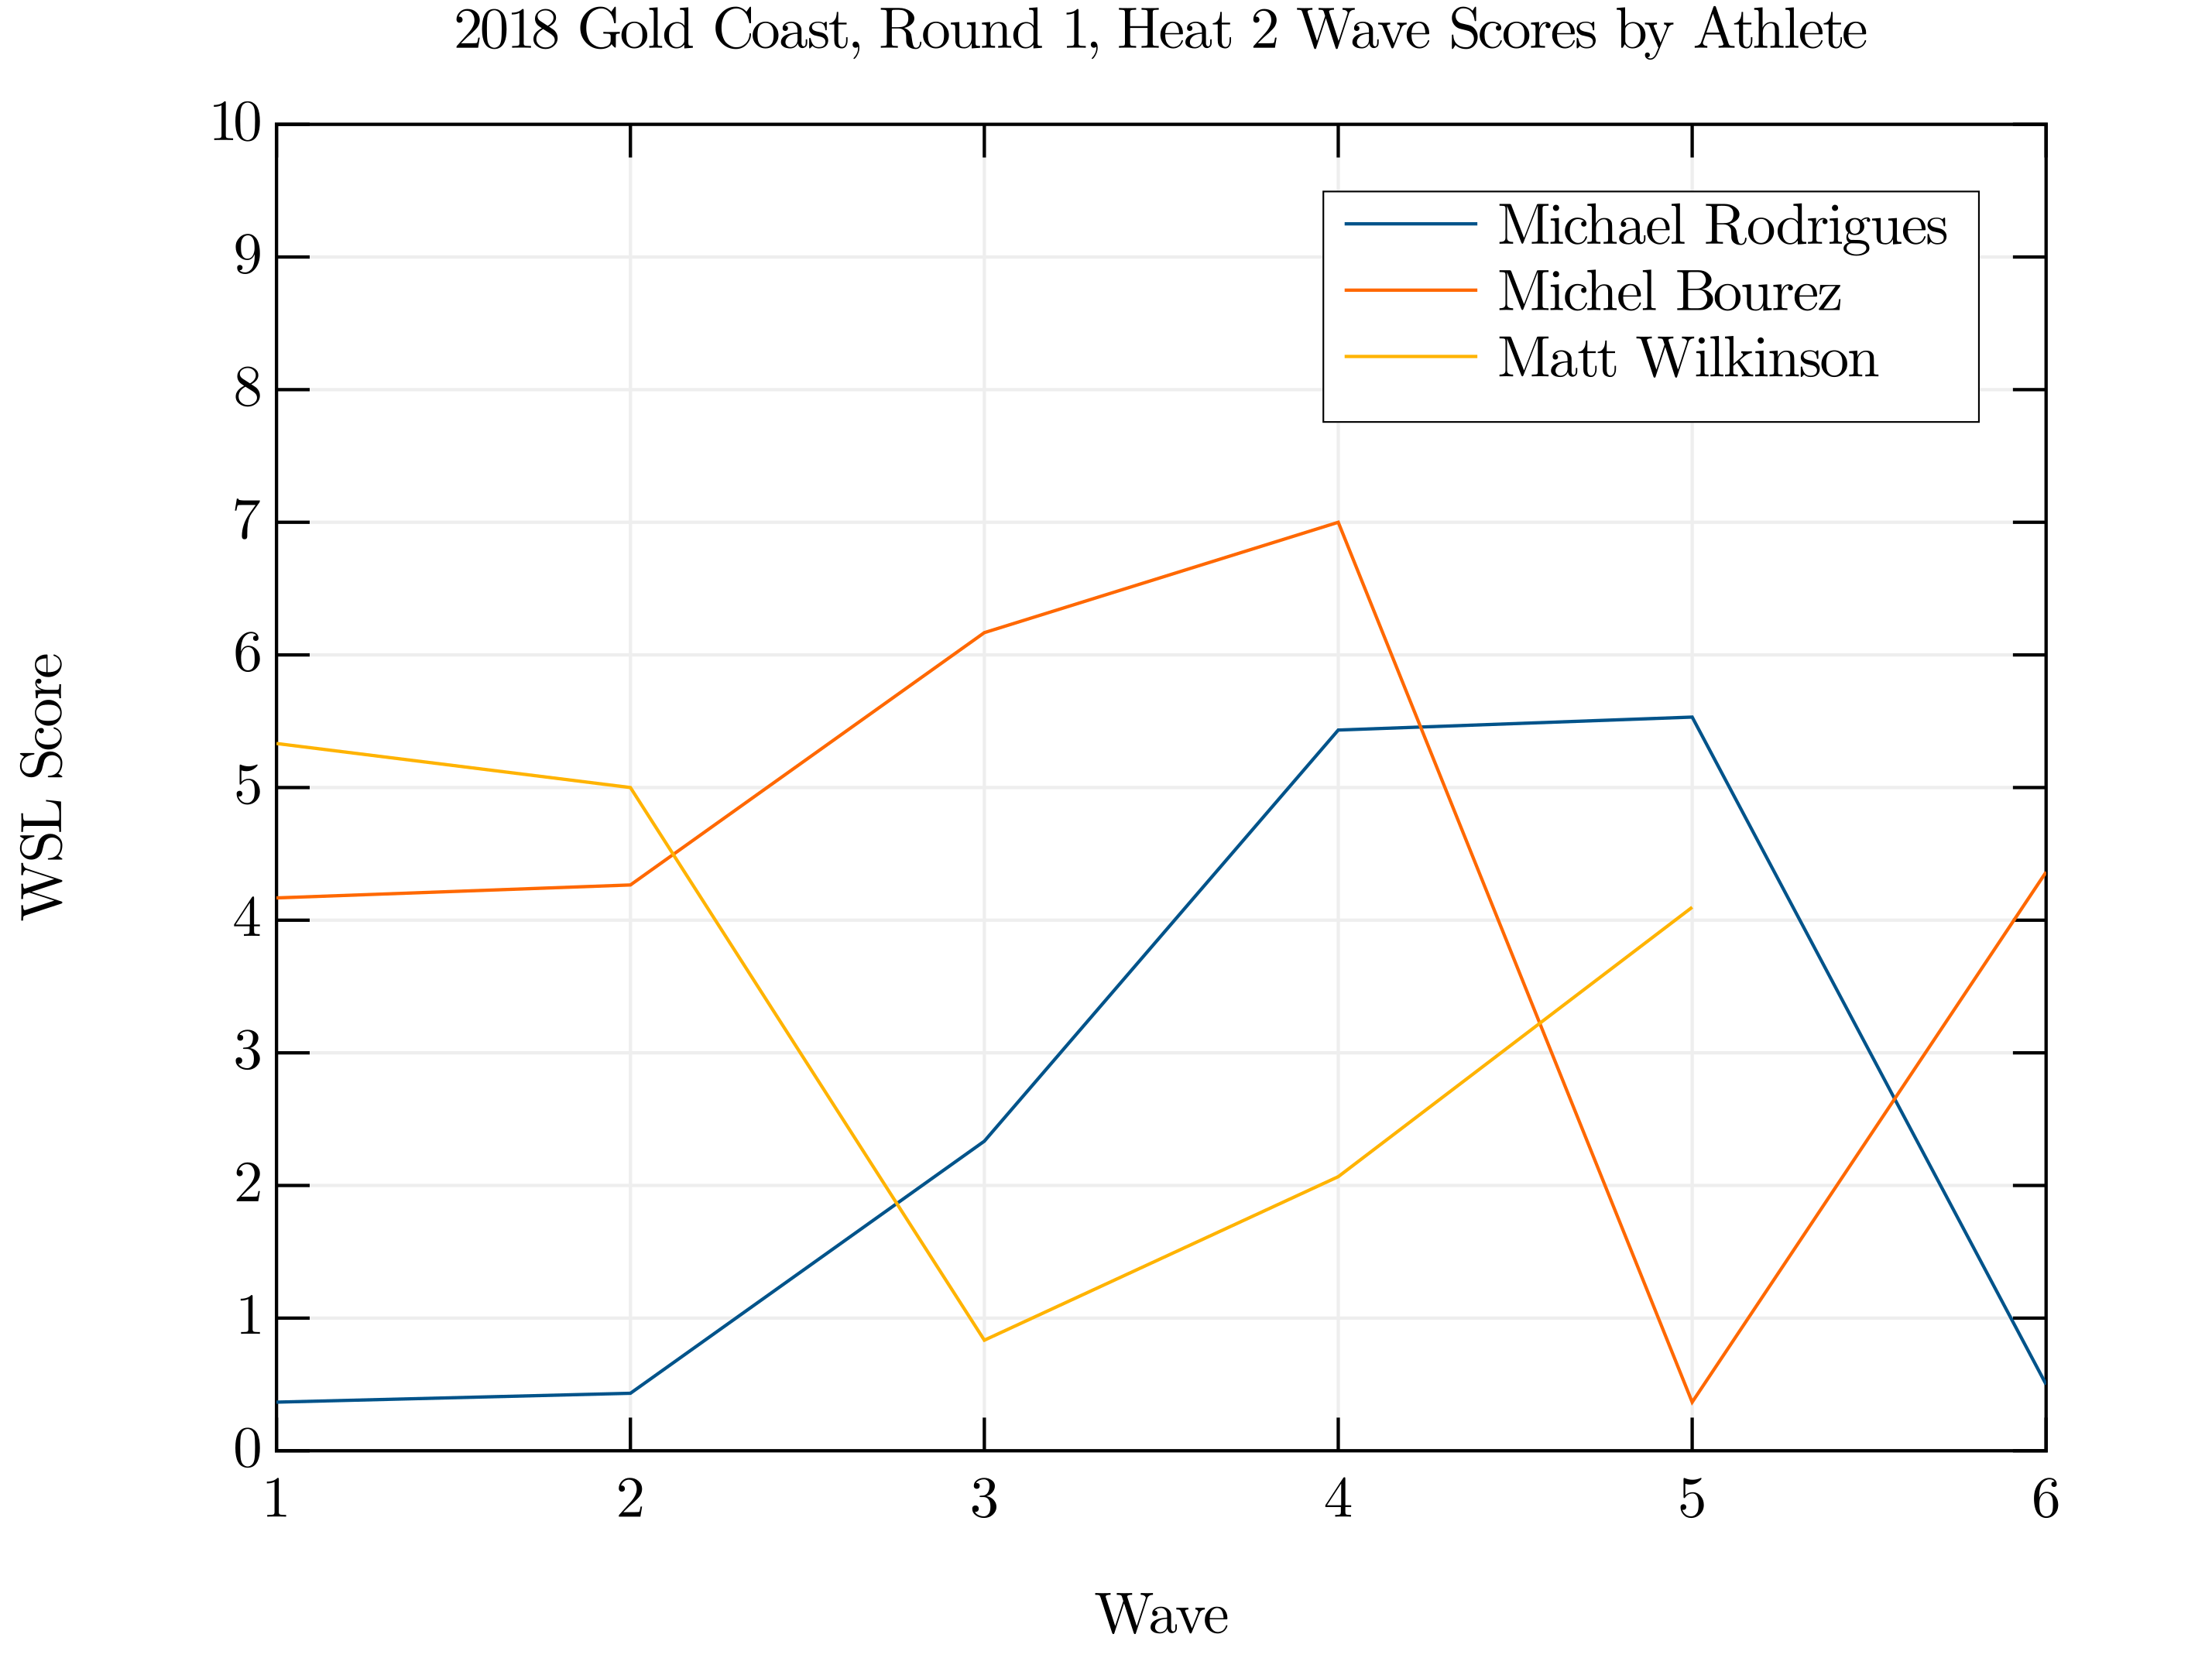
\includegraphics[width=6cm]{./src/visuals/2018GCR1/WaveScoresByAthH2.png}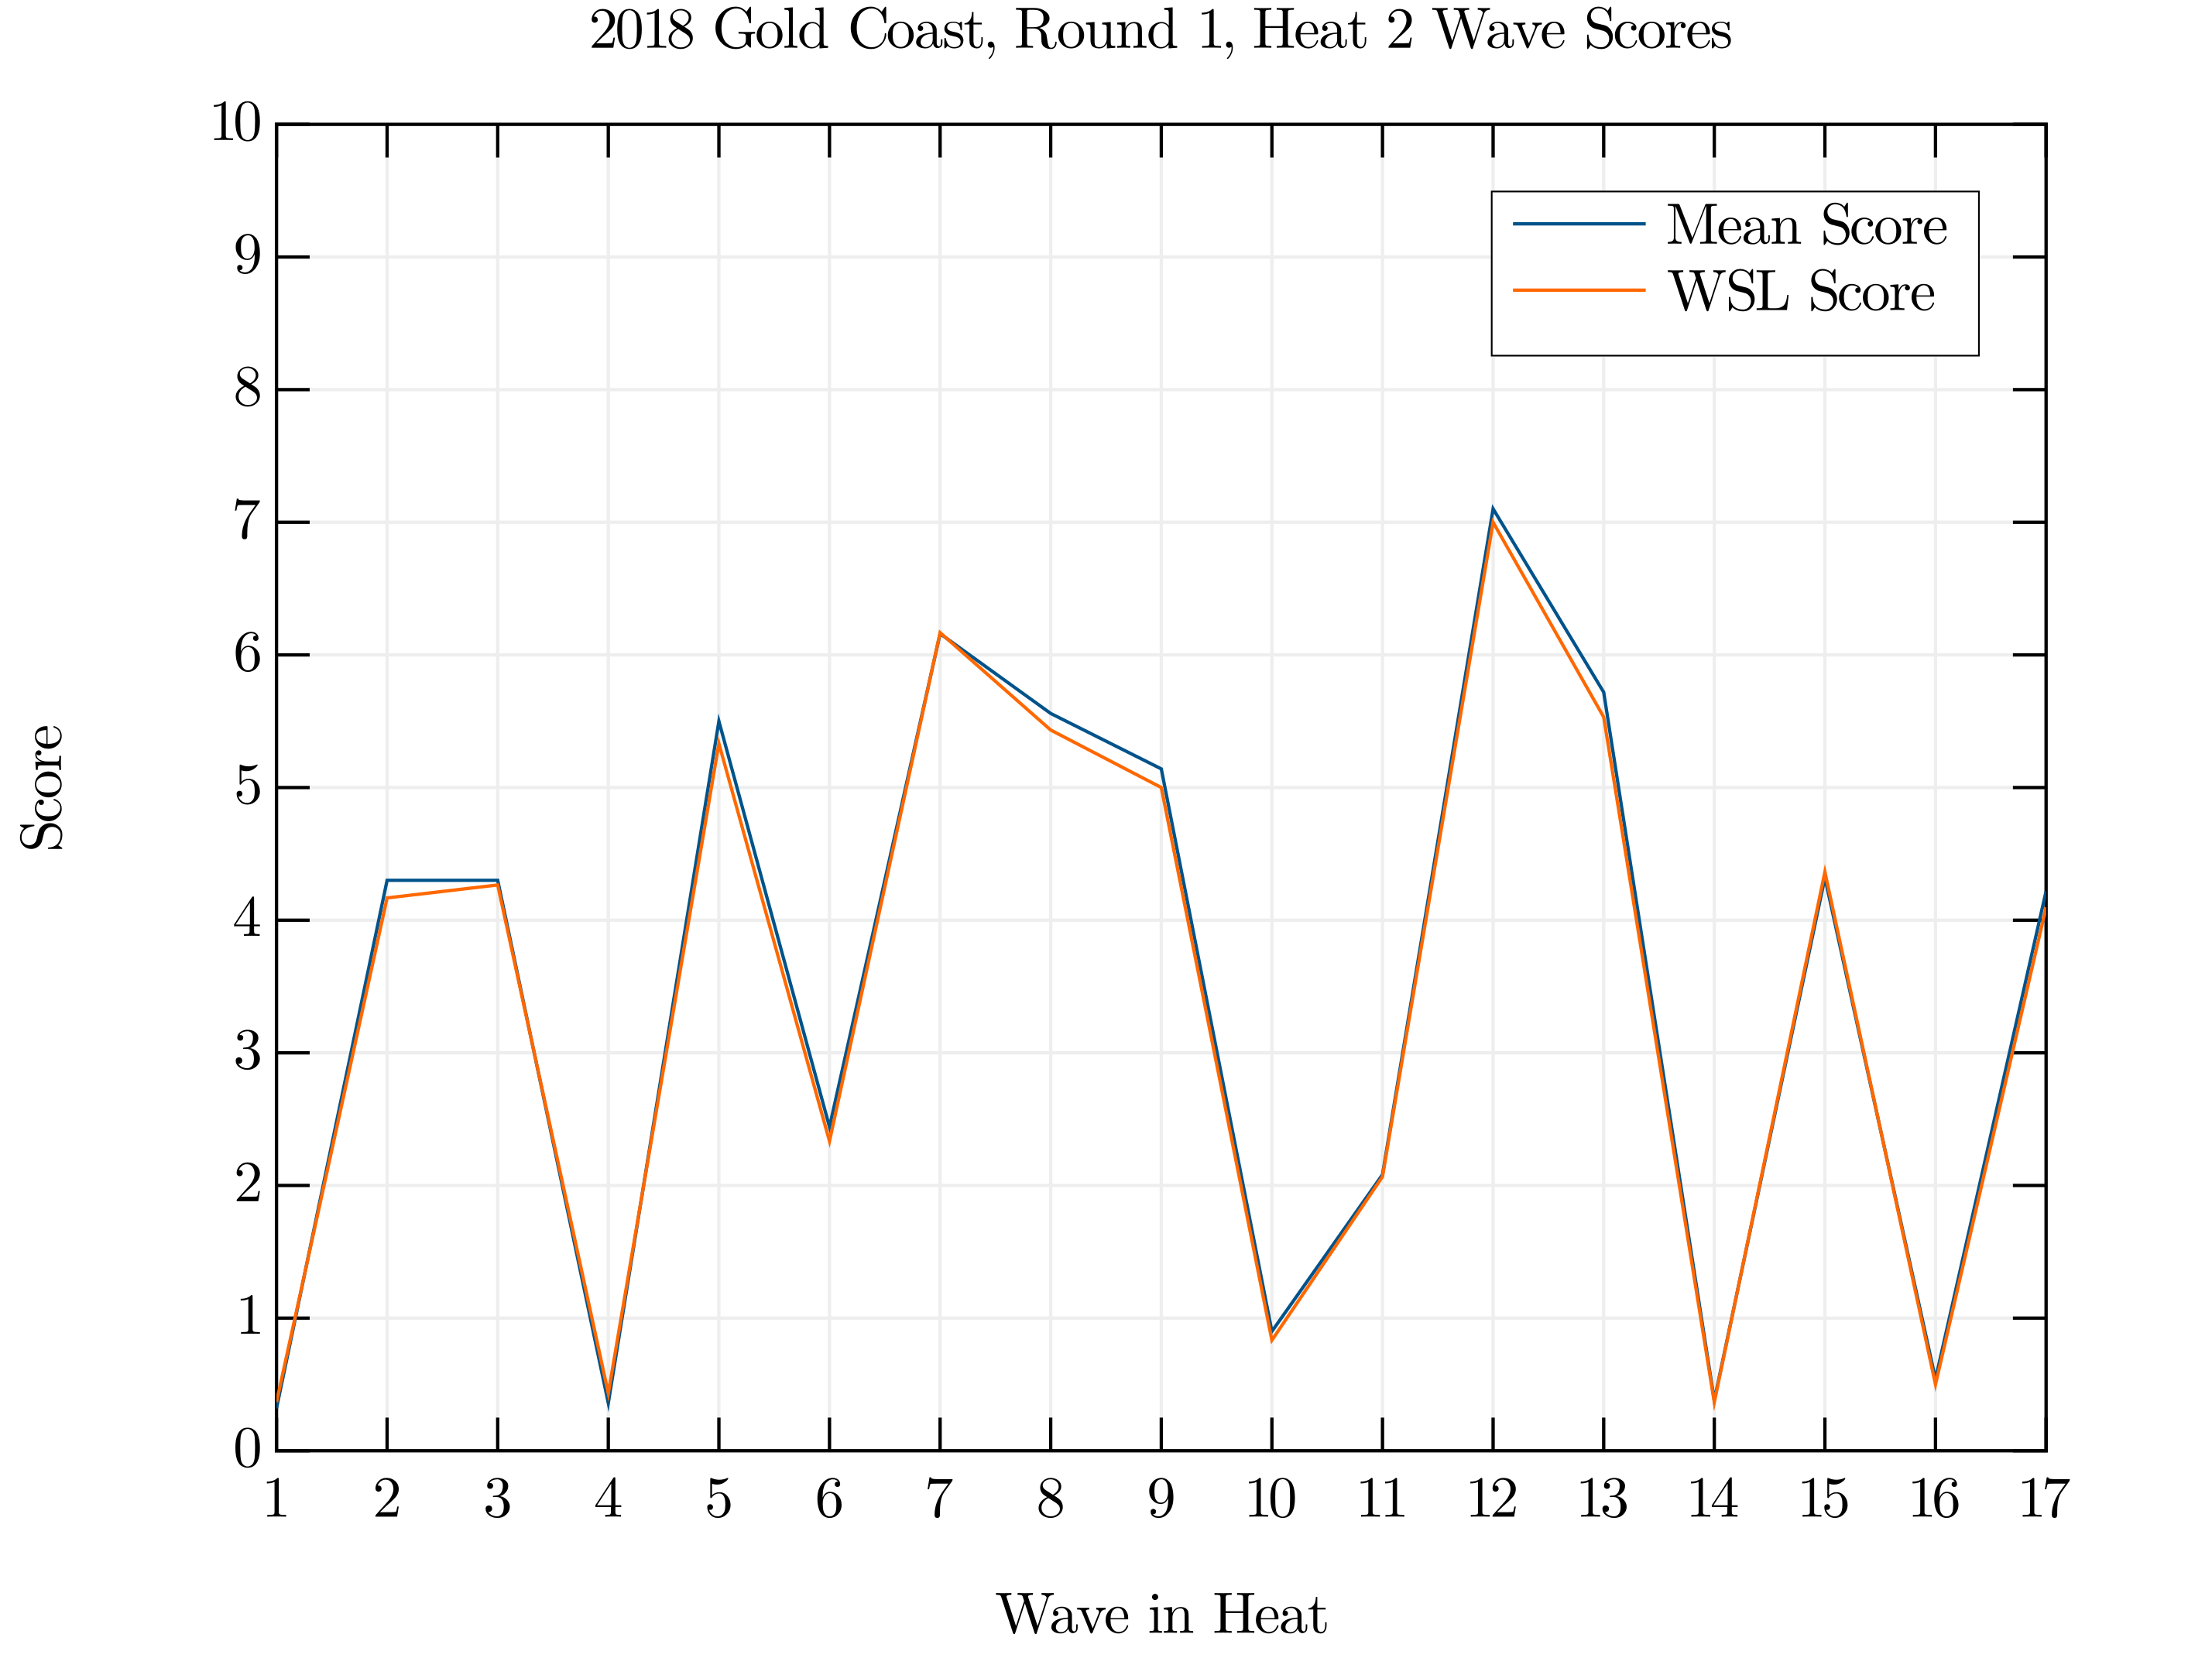
\includegraphics[width=6cm]{./src/visuals/2018GCR1/WaveScoresH2.png}


There's a couple characteristics of these heats that are emblematic of the various w


\subsection{The Judging Process}
Though there are 5 judges and 5 scores, the score a surfer receives, called the "wave score", is the trimmed mean of the scores given by the 5 judges. This is very important information and particularly interesting because it distinguishes the \textit{existence} of biased judges from the effect of biased judging (if it exists).

The role of judges is not limited to the five judges on a panel. For each Men's CT event, there is 1 international Head Judge, 7 international judges, and 1 international priority Judge (Chapter 13, Article 179.01). And Chapter 13, article 179.17 states that "At CT Events, the number of judges from any one regional area is limited to 3". For each heat, the WSL Head Judge must assure there are at least 5 judges on the panel for each heat and that they are a subset of the 7 International Judges and 1 International Head Judge (Chapter 13, Article 179.13).

Note: that Different elements of this list may be emphasized more or less depending on the location, conditions, and changes of conditions. (Chapter 13 Article 182) Additionally, the General Judging Rules (Chapter 13; Article 183; Section 1,2) state that judges should be visually separated, should not discuss scores, and may not change their scores.

Though there is no formal rubric for judging, the following criteria are emphasized.
\begin{itemize}
\item Commitment and degree of difficulty
\item Innovative and progressive maneuvers
\item Combination of major maneuvers
\item Variety of maneuvers
\item Speed, power, and flow
\end{itemize}
Since there are a wide range of locations or wave conditions, the relative importance of an element on this list will vary. The elements of that the judges believe are particularly important on a given day are sometimes communicated to surfers and viewers.

\subsection{The Panel Data}


JOJO: Can you just pick one (or maybe two) heats to use as running examples please? What heat characteristics would we like here. We don't have to look too far.

There are many beautifully intricate parts the data, but this one caught our interests.
Question: What is the definition of a panel? What type of data is it?
For any given heat, there are 5 judges on the judging panel. Anytime a surfer rides a wave, each of them independently observes the wave and writes down a score. 

What does a panel look like? A lot of very different things that may seem very similar BUT ARE NOT. For example:

The most granular object of study is the panel. It would not be justified to analyze our data a sequence of 13,872 panels because during each heat the set of judges is fixed (or at least it appears to be this way).

For this reason we will be mostly interested in heat-level dynamics of the panel. This is similar to the game-level approach Price takes in analyzing NBA refereeing (as opposed to simply many foul calls). A panel is comprised of a set of distinct humans, called judges. We denote the set of judges as $J=\{j_1, j_2, j_3,j_4, j_5\}$, and their origins by the multiset $J_c:C\rightarrow\mathbb{N}$. Multisets are interesting. Roman defines a multiset on a set A, as an element of A×N. Blizzard gives in broad overview of different approaches to multisets in [The Development of Multiset Theory], and takes a more normative approach in [Dedekind Multisets and Function Shells]. We will not delve into this, but they are important to understand in the construction below:

A definition: A multiset on a set A, is a function $f:A\rightarrow\mathbb{N}$.

Some authors use the pair (A,f) to define a multiset. While it may bring us comfort to know the underlying set which the function is defined on, this is merely a luxury of defining a multiset. In an observational setting one does not necessarily know the underlying set, only the support of f, i.e. the set of all elements mapped to a non-zero number. For example, the judges in a heat are selected from a pool of judges provided by the WSL for that event. Specifically, suppose it is march 
%___
2018, Caio Ibelli rides the first wave of the WSL 2018 Men's Championship Tour, when all 5 judges provide their scores, Caio Ibelli is awarded a score of:
%round(mean(sort(WAVES[1][2].judge_scores)[2:4]),digits=2)
Not a dramatic first wave eh? But maybe you want to know a bit more about the sub scores that resulted in a wave score of 0.43 . The panel is as follows:
%WAVES[1][2].panel
We can certainly deduce the nationalities of 5 of the 8 Judges in the event pool.
%WAVES[1][2].panel_origs

Where are the remaining 3 judges from? Well, we have to wait for the next heat because these judges are the panel for this heat. In the next heat, Michael Rodrigues is the first to ride a wave, receiving a 0.3.
%round(mean(sort(partitionBy(:heatId)[2][2][1].judge_scores)[2:4]),digits=2)
This feels similar to the first wave of last heat, are the judges the same?
%partitionBy(:heatId)[2][2][1].panel
Looks like No. Okay, well are some of them the judges the same? Certainly. We could have answered that even before the Caio Ibelli took the first wave of 2018 because if there were two panels, each with five judges, and no judges were the same, then there would be at least 10 total judges for the event, a breach of WSL rule book. So, which of the judges from heat 1 are on the panel from round 2?
we know there are at least:
[AUS => 2, BRA => 2, ESP => 1, USA => 1, ZAF => 1]
 If we assumed the panels were disjoint, we could deduce that the pool of judges for the event, at least, consisted of:
println([AUS => 3, BRA => 3, ESP => 1, USA => 2, ZAF => 1])
However, our information from the rule book tells us that this certainly cannot be the case.

\subsection{Multisets}
Though the definition of a multiset on A as a function $f:A\rightarrow\mathbb{N}$ is pleasant to work with, it omits some of the structure intrinsic to a multiset. Namely, consider how a multiset arises in an applied setting. We have some knowledge or information about the judges, ie. some function $k: J_{pool} → C$, which maps a judge in the judging pool to their nationality $c\in C$. How do we arrive at the $f:C\rightarrow\mathbb{N}$ ? By: $f(c) = \sum_{j\in J} 1_{k(j)=c}$. Evidently f is the sum of simple functions of our information. So f really isn't representative of much and truly depends on some reference set or information. Additionally, if we had additional structure on J, for example a total order where $j_1<j_2<j_3 <j_4<j_5$, its not entirely clear how we can extend the structure to the multiset.



$M(A)$ may be understood as an unordered array. Suppose we have a set $A = \{x,y,z\}$, then 
$l(A) = \{ () \}\cup \{(x),(y),(z)\} \cup \{(x,x)(x,y),(x,z),(y,x),(y,y),(y,z),(z,x),(z,y),(z,z)\} \cup \dots $
$M(A) = \{()\}, \{(x)\},\{(y)\},\{(z)\} , \{(x,x)\}, \{(x,y),(y,x)\},  \{(x,z),(z,x)\},\{(y,y)\},\{(y,z),(z,y)\}, \dots $

We introduce array notation, in which the multiset $\{(x,x,y),(x,y,x),(y,x,x)\} = [x,x,y]$ or equivalently as $[x,y,x]$, $[y,x,x]$. More formally we define an array $[ma^1,ma^2,\dots, ma^k] := S_k(ma^1,ma^2,\dots,ma^k)$


Hence, we define: a multiset on a set A is \textbf{an} equivalence class of $l(A)$ where:
$l(A):= \bigcup_{n\in\mathbb{N}}A^{×n}$ where ×n denotes the nth Cartesian power. Note that this is certainly a disjoint union.
$M(A) := l(A)/\sim$ where $x\sim y$ if and only if $\#x=\#y $ and $\exists \tau \in S_{\#x}$ s.t. $\tau x=y$, where $\#x:=n $ s.t. $ x\in A^{×n}$. 
To show that $M(A)$ is well defined, we must show that $\sim$ is an equivalence relation:
\begin{itemize}
\item Claim: $x\sim x$. PF: $ e \in S_{\#x}$ so ex = x and $\#x=\#x$, thus $ x\sim x$.
\item Claim: $ x\sim y \implies y\sim x$. PF: Assume $x\sim y$, i.e. $\#x = \#y$ and $ \exists \tau \in S_{\#x} $ s.t. $\tau x = y$. So, $S_{\#x}=S_{\#y} \implies \tau^{-1} \in S_{\#y}$, and $\tau^{-1}y = \tau^{-1}\tau x = ex = x$. And we have $ \#y=\#x$, thus $y\sim x$.
\item Claim $ [x\sim y \:\And\:  y \sim z] \implies x \sim z $.Assume $x\sim y$ and $y\sim z$. $\#x=\#y$ and $\#y=\#z$ implies that $\#x=\#z$ and $S_{\#x}=S_{\#y}=S_{\#z}$. By assumption $\exists \tau, \gamma \in S_{\#x}$ s.t. $\tau x=y$ and $\gamma y=z$. So $z = \gamma y = \gamma \tau x $ and $\gamma\tau \in S_{\#x}$. Thus, $x\sim z$.
\end{itemize}

Further, let us define:
$\otimes:l(A)\times l(B)\rightarrow l(A\cup B)$ by $\otimes(x,y):=x\otimes y $, i.e. $ \otimes((x^1,\dots,x^m),(y^1,\dots,y^n)) =  (x^1,\dots,x^m)\otimes(y^1,\dots,y^n) =(x^1,\dots,x^m,y^1,\dots,y^n)$. This is well defined because $x\otimes y \in (A\cup B)^{\times(m+n)} \subset l(A\cup B)$. This may be interpreted as 
And define $\otimes:M(A)\times M(B)\rightarrow M(A\cup B)$  by $\otimes(mA,mB):=\{\otimes(x,y) \mid (x,y)\in mA\times mB\} = \{x \otimes y \mid (x,y)\in mA\times mB\} = mA\otimes mB$

To be clear: \textit{$M(A)$ is a set of equivalence classes of $l(A)$ under $\sim$,} and a multiset on A, denoted mA, is an element of $M(A)$, i.e. mA is an equivalence class. Though $(mA^1,\dots,mA^k)$ and $\otimes(mA^1,\dots,mA^k)=mA^1\otimes\dots\otimes mA^k$ look very similar, they are not the same.
\begin{itemize}
\item $(mA^1,\dots,mA^k)$ is a k-tuple of multisets on A which means it is an element of $M(A)^{\times k}$ and thus an element of $l(M(A))$ because $M(A)^{\times k} \subset l(M(A))$.
\item $\otimes(mA^1,\dots,mA^k)=mA^1 \otimes\dots\otimes mA^k$ is not in $M(A)$, rather it is a subset of an element of $M(A)$, specifically, $mA^1 \otimes\dots\otimes mA^k \subset \{ \tau x \mid  x\in mA^1\otimes\dots\otimes mA^k \:\text{and}\: \tau \in S_{\#x} \} = mA \in M(A)$.
\end{itemize}
This construction has some nice properties:
\begin{itemize}
\item The automorphism of  a multiset, $mA$, is $S_{\#mA}$ (where $\#mA := n $ s.t.  $mA \subset A^{\times n}$).
\item Let $V_A := span\{e_a \mid a \in A\}$ over $\mathbb{R}$ (any field with char 0 should do i think). Given any function $\alpha:M(A)\rightarrow\mathbb{R}$ we may define $v \in T(V_A)$ by $v = \sum_{W \in M(A)} \alpha(W) \sum_{w\in W}v_w$, which is completely symmetric by definition of W ($v_w = e_{w^1}\otimes\dots\otimes e_{w^{\#w}}$)
\item Any $p:mA\rightarrow\mathbb{R}$ satisfying $\sum_{t\in mA} pt = \sum_{t\in mA} p(t^1,\dots,t^{\#t}) = 1$, defines a probability distribution. Moreover, we may represent this as some $P \in T(V_A)$ by defining $P=\sum_{t\in mA} ptv_t = \sum_{t\in mA} p(t^1,\dots,t^{\#t})v_t $. (In general we will not place parenthesis around a functions argument).
\item With the same p as above, we may define a polynomial $F\in \mathbb{R}[x_a \mid a \in A]$by $F(x_1,\dots,x_{|A|}) = \sum_{t\in mA} ptz_t$ where $z_t $is the monomial: $\prod_{a\in A} x_a^{t_a}$ where $t_a := |\{j \mid t^j = a\}|$
\end{itemize}

\begin{definition}: An \textbf{ordered partition} of a multiset mA is a k-tuple of multisets on A, $\lambda=(mA^1,\dots,mA^k)$, satisfying $\otimes\lambda=\otimes(mA^1,\dots,mA^k)=mA^1\otimes\dots\otimes mA^k \subseteq mA$. And by definition of $\#, \#\lambda=k$. \end{definition}
\begin{definition}: The set of ordered partitions of a multiset $mA\in M(A)$ is $\Pi_{mA}:=\{\lambda \in l(M(A)) \mid \otimes\lambda \subseteq mA\}$. \end{definition}
\begin{definition}: An unordered partition of a multiset mA, is a multiset of multisets on A, i.e. some $K \in M(M(A))$, satisfying $k\in K \implies \otimes k \subseteq mA$. By definition of multiset, $K=\{ \tau k \mid \tau \in S_{\#k}\}$.\end{definition}
\begin{definition}: The set of unordered partitions of a multiset $mA \in M(A)$ is $\Upsilon_{mA} := \{ U \in M(M(A)) \mid \upsilon \in U \implies \otimes\upsilon \subseteq mA \}$.  In English this is precisely saying that the set of unordered partitions is a set of multisets of multisets, each of which is an unordered partition of a particular multiset,$mA$.\end{definition}

\begin{definition}: A multiset mA is a sub-multiset of mB if and only if 
\end{definition}


\begin{remark} These look and sound a bit absurd at first, however, they are the proper definitions. We introduced If you replace "multiset" with "set, we end up with:
The set of ordered partitions of a set A is a set of k-tuples, each of which partitions A.
The set of unordered partitions of a A is a set of sets of sets, each of which is a unordered partition of A.
\end{remark}

JOJO can you show that the function definition by blizzard is a faithful representation of this ?? that would be useful. Think slowly here Representation in a discrete set function space should be the same thing that you understand concretely in GL(V).

\subsubsection{Various actions of permutations}
The actions of permutations on different mathematical objects can be a bit confusing. We desire to be clear and consistent with our notation:
\begin{itemize}
\item $\tau \in S_d= S_{\{1,\dots,d\}}$ acts on the set $\{1,2,\dots,d\}$ by acting on the elements of the set $\tau\{1,2,\dots,d\} = \{\tau(1),\tau(2),\dots,\tau(d)\}$.
\item $\tau\in S_d$ acts on d-tuples by permuting the \textbf{positions} of the entries.
\item When we wish to discuss a permutation acting on the \textbf{elements} of an n-tuple, we will write $\hat{\tau}$, formally $\hat{\tau}:\{1,\dots,d\}^{\times n} \rightarrow \{1,\dots,d\}^{\times n}$ and is defined by $\hat{\tau}(z_1,z_2,\dots,z_n) := (\tau(z_1),\tau(z_2),\dots,\tau(z_n))$.
\end{itemize}

For a concrete example let $d=3, x=(USA,AUS,BRA), y=(1,1,2)$ and 
$$\tau = \begin{pmatrix} 1 & 2 & 3\\ 3 & 2 & 1 \end{pmatrix}$$
$\tau$ acts on by x by rearranging the entries of x, i.e. $\tau x = \tau(USA,AUS,BRA) =(BRA,AUS,USA)$. $\hat{\tau}$ cannot act on x because $\tau$ is not defined on $\{AUS,BRA,USA\}$.
$\tau$ acts on by y by rearranging the entries of y, i.e. $\tau y = \tau(1,1,2) =(2,1,1)$. $\hat{\tau}$ acts on y by applying $\tau$ to each entry of y, i.e. $\hat{\tau}y = \hat{\tau}(1,1,2) =(\tau(1),\tau(1),\tau(2) ) =(3,3,2)$.

\subsection{Partitions And Exchangeability}
This notion of a partition is different than the typical ones. P Martin and others use a Partition Algebra first introduced by Brauer in 1913?, we are no experts in this realm but the notion seems most useful when analyzing the automorphisms of partitions of a set. Multisets cannot be accommodated (JOJO you must be more informed than this come on man).

A more statistical interpretation of partitions appears in a seminal paper on population genetics by Kingman in 1978 (Random Partitions in Population Genetics). More abstract interpretations come in a later paper (The Representation of Partition Structures). The partitions defined are integer partitions (which is the typical interpretation, see also Vershik's paper Statistical Mechanics of Combinatorial Partitions and Their Limit Shapes). Integer partitions are no different than **set** partitions, one can pass freely between the two by taking the carnality of sets, with one assumption: that the elements of the set are exchangeable. This is defined in Pitman's 1995 paper, (Exchangeable and Partially Exchangeable Random Partitions). "Partial Exchangeability" is a very intuitive notion. Consider a random variable, $\lambda$, which takes values in the set of ordered set partitions of $\{1,\dots,n\}$, denoted $\Pi_n$. And consider its probability distribution, $p:\mathbb{\Pi}_n\rightarrow\mathbb{R}$.  $p$ is partially exchangeable iff. $\forall \lambda \in \Pi_n \forall \tau \in S_{\#\lambda} \quad p(|\lambda^{1}|,\dots,|\lambda^{\#\lambda}|) = p(|\lambda^{\tau^{-1}(1)}|,\dots, |\lambda^{\tau^{-1}(\#\lambda)}|)$. In English, this means that the probability of observing some ordered partition with $\lambda_1$ blocks of size 1, $\lambda_2$ blocks of size 2, …, $\lambda_n$ blocks of size n is the same regardless of the order of the blocks (to be clear $\lambda_k := |\{k \mid  |\lambda^j| = k \}|$). This defines \textbf{part}-ial exchangeability.

The definition of plain old exchangeability is distinct. A random partition $A \in \Pi$ is exchangeable if and only if $p(A) = \hat{\tau}p(A) \quad \forall \tau\in S_n$.

Recall:
Let $\tau \in S_k$. How does $\tau$ act on $(A^{1},\dots,A^{k})$ ? By $\tau(A^{1},…,A^{k}) = (A^{\tau^{-1}(1)},\dots,A^{\tau^{-1}(1)})$, i.e. moving $i^{th}$ argument to the $\tau(i)^{th}$ position. So it makes sense to define $\tau\otimes(A^{1},\dots,A^{k}) = \otimes(A^{\tau^{-1}(1)},\dots,A^{\tau^{-1}(k)})$ because we have defined it that way for functions, and $\otimes$ is a function.

In the case of the first wave of 2018, ridden by Caio Ibelli: $A=(\{BRA, ZAF\},\{ESP, AUS, USA\})$ and $A \in \Pi_{\{AUS,BRA,ESP,USA,ZAF\}}$. So $\tau:=(1 2)\in S_2$, acts on A by $\tau(\{BRA, ZAF\},\{ESP, AUS, USA\}) = (\{ESP, AUS, USA\},\{BRA, ZAF\})$.

Pitman calls this the "natural action of permutations of $\{1,…,n\}$  on $\lambda$ and refers to earlier references by Kingman and a delightful survey of exchangeability by Aldous (Exchangeability and related topics)(we have altered the quote to use {1,…,n} instead of Pitman's $N_n$). The "natural action" of permutations of a set X on a partition of X is a subjective notion. We agree Pitman's thinking here and are fans of the chapeau. 
In practice this looks like taking some $\gamma \in S_{\{AUS,BRA,ESP,USA,ZAF\}}$. 
\[\gamma=
\begin{pmatrix} 
\text{AUS} & \text{BRA} & \text{ESP} & \text{ESP} & \text{ZAF}\\
\text{BRA}  & \text{ESP} & \text{ZAF} & \text{AUS} & \text{ESP}
\end{pmatrix}
\] (this is arbitrary choice). 

\(
\begin{pmatrix}
1 & 2 & 3\\
a & b & c
\end{pmatrix}
\)

$ \hat{\gamma}(\{BRA, ZAF\},\{ESP, AUS, USA\}) =(\gamma\{BRA, ZAF\},\gamma\{ESP, AUS, USA\}) $
$ =(\{\gamma(BRA),\gamma(ZAF)\},\{\gamma(ESP),\gamma(AUS),\gamma(USA)\}) = (\{AUS, ESP\},\{ZAF, BRA, AUS\}) $

In this concrete setting, the definition of exchangeability requires that $P(\{BRA,ZAF\},\{ESP,AUS,USA\}) = P(\{\gamma(BRA),\gamma(ZAF)\},\{\gamma(ESP),\gamma(AUS),\gamma(USA)\})$ for every permutation $\gamma$ of $\{AUS,BRA,ESP,USA,ZAF\}$. If the distribution over ordered panels is exchangeable, then we can assert: the probability of any arrangement of judges is equal to the the probability of that arrangement under any permutation of judge labels. Further analysis would be required to see if this holds conditional on a surfer's country. But is this the right notion of exchangeability that we are after?

Remember the first wave of the second heat of 2018? Michael Rodrigues started the heat of with a whopping 0.3, but taking the panel the under an equivalence relation that Judge1 $\sim$Judge2 if and only if Judge1's score = Judge2's score, we ended up with an ordered partition of the panel: $([BRA],[AUS,AUS,USA],[BRA])$. Our desired exchangeability is: $P([BRA],[AUS,AUS,USA],[BRA]) = P\hat{\gamma}([BRA],[AUS,AUS,USA],[BRA])$

Taking a similar $\gamma:=\begin{pmatrix} AUS & BRA & USA \\ BRA & USA & AUS \end{pmatrix}$ as before, $P(\gamma[BRA],\gamma[AUS,AUS,USA],\gamma[BRA])= P([\gamma(BRA)],[\gamma(AUS),\gamma(AUS),\gamma(USA)],[\gamma(BRA)])$ = $P([USA],[BRA,BRA,AUS],[USA])$. This seems a little hard to expect, at least within our heat, because the panel for this heat consists of 2 Australian judges, 2 Brazilian judges, and 1 American judge. Or maybe we would like to be strict and require that arrangements, with their multiplicities, are equally probable under any permutation of judge origins?

(JOJO i need you to be able to pin down when this is a "fair" or somewhat "fair" expectation and when it is not. Does this necessitate that countries are equally represented? Yes i think, if we are seeing ordered arrangements of our full multiset, but no if we are seeing ordered arrangements of a subset of the multiset, for example, we could have exactly 5 judges of each country. But it is also viable if we have >= 5 judges from each ctry. How does the definition change when we use $\gamma\in S_{ctry set}$ vs. $\gamma\in S_5$? Generalizing this seems incredibly fun.   .... Thinking about this a bit more, we could just frame everything in terms of orbits of a multiset mA or partition of mA, which depends on the group of choice. If we take $S_{\#\lambda}$ as the group, the orbit of some $\lambda \in \Pi_{mA}$ is the set of permutations of the blocks. If we take the group to be $S_C$, the orbit of $\otimes\lambda$, (under applications of $\hat{\gamma}$), will be the permutations of frequencies of element of the multiset. Note that if we take $\lambda$ alone, we must apply $\hat{\hat{\gamma}}$ for $\gamma \in S_C$. Now, what if we take a combined orbit?)

Regardless of whether this is a fair notion, you may notice that we passed the action of $\gamma $ to the elements of our multiset, without justification. This is not justified. Nor have we defined anything that would work this way (yet).These are the difficulties with multisets that motivate our definitions and a lot of the interest in these panels.

\subsection{Definitions Of Exchangeability}
A probability distribution on multiset partions $P: \Pi_{mA}\rightarrow \mathbb{R}$ is.....
\textbf{Partially exchangeable} if and only if: 	$\forall \lambda \in \Pi_{mA}\:  \forall\tau\in S_{\#\lambda} \quad P\lambda =P\tau\lambda$, i.e. $P(mA^1,…,mA^k)= P\tau(mA^1,…,mA^k) $

\textbf{Exchangeable} if and only if:
$\forall \lambda \in \Pi_{mA}\:\forall \gamma\in S_n\quad P\circ\otimes\lambda=P\circ\gamma\circ\otimes\lambda $ where $n:=\sum_k k\lambda_k$ (note that $\gamma$ is applied to elements of $\otimes\lambda$ which are all n-tuples so action of $S_n$ makes sense.

\textbf{Label exchangeable} if and only if $\forall \lambda \in \Pi_{mA} \: \forall \beta \in S_A \quad P\circ\otimes\lambda = P\circ\hat{\beta}\circ\otimes\lambda$ 

\textbf{Intra-multiplicity exchangeable} if and only if 
$ \forall \lambda \in \Pi_{mA} \forall \beta \in \prod_{k=1}^{\#mA} S_{\lambda_k} \quad P\otimes\lambda=P\hat{\beta}\otimes\lambda$

and for $\omega\in\otimes\lambda, \hat{\beta}\omega=\hat{\beta}(\omega_1,\dots,\omega_n) = (\beta\omega_1,\dots,\beta\omega_n)$.

I have a bag of judges from in 2018 or 2019
%(Y_2018 bag for 2018, Y_2019 bag for 2019)
%((evt1 bag, …,evt11 bag), (evt1 bag,…,evt11bag))

%given pool = (n_AUS,n_BRA,n_ESP,n_FRA,n_PRT,n_USA,n_ZAF)
%given panel = (k_AUS,k_BRA,k_ESP,k_FRA,k_PRT,k_USA,k_ZAF)

%P(Heat | Panel ) = (1/#waves∑(k_AUS!k_BRA!k_ESP!k_FRA!k_PRT!k_USA!k_ZAF / 5!)∏1/λ_i!) 
%P(Heat | Panel ) = (1/(n_AUS)(n_AUS-1)…(n_AUS-k_AUS))⋅…⋅(1/(n_ZAF)(n_ZAF-1)…(n_ZAF-k_ZAF))(1/#waves∑(k_AUS!k_BRA!k_ESP!k_FRA!k_PRT!k_USA!k_ZAF / 5!)∏1/λ_i!) 

JOJO how bout we implement a multivariate-hypergeometric model for panel composition, you can use multinomial prior, and i think you can probably get marginals that look like multinomials, but you will have some vector p corresponding to ORIG concentration to estimate, but i think we know what p is empirically for almost every event. So we should be able to assess deviations from our expectations, or just do this fully bayesian (but then we'd end up with a result for an estimate of a quantity we already know... in most cases.)

JOJO How bout you actually just make a quick through all of the rank tests you know / can find. they really aren't too hard to code, just do it. Then we can see how well they do, and maybe improve upon them? Figure out WHY they work or don't work.

\subsection{Lets talk about equivalence classes and the axiom of choice}

\subsection{Cumulants}
These seem to be considered mostly when the random variable is a number or a vector. We do not have either of those.
Propose: Cumulant of a tensor (of rank d) defined by automorphisms, which we could consider as measurable maps. Just as the first cumulant of a vector is defined by the first moment, this can be the case for a tensor. 

Some citations:
T.P. Speed Cumulants and Partition Lattices I,II, ...



\section{Methods}
Throughout:
$M = \{Match,Non-Match\} = \{M,\neg M\}$. $C = \{AUS,BRA,ESP,FRA,PRT,USA,ZAF\}$. $D = \{1,\dots,d\}$
$V_M := \{e_{Match},e_{Non-Match}\} $, $V_C = \{ e_{AUS},e_{BRA},\dots,e_{ZAF} \}$

Lets explore the Data!
We have lots of missing Judge Origins from panels in the 2017 World Surf League season so we will omit the 2017 season ... for now (This begs an interesting question which we should return to later). We have constructed a multidimensional array, aka an m-way, cross classified, contingency table. We have m classification factors:
\begin{itemize}
\item WSL Season
\item Event
\item Round
\item Heat
\item Ahtlete Origin
\item Judge Origin
\item Size of Partition of Panel (Max Rank)
\item Rank of Judge
\end{itemize}


\subsection{Symmetric Group}
\begin{definition}When G is a Group, and $\mathbb{F}$ is a Field, the Group Algebra of G over $\mathbb{F}$, denoted $\mathbb{F}[G]$, is the space of formal linear combinations of elements of G. Elements of $\mathbb{F}[G]$ are of the form: $c_1 g_1 + \dots + c_n g_n = \sum^n_{i=1} c_i g_i$, where $c_i \in \mathbb{F}, g_i \in G$. Note that $i\neq j \implies g_i \neq g_j$ because G is a set of elements, so no element occurs with multiplicity. For example, $c_1 g + c_2 g \not\in \mathbb{F}[G]$ whereas $(c_1 + c_2)g \in \mathbb{F}[G]. $\end{definition}

\begin{remark} $\mathbb{F}[S_d]$ is comprised on formal linear combinations of elements of $S_d$. A generic element, $A \in \mathbb{F}[S_n]$ looks like, $\sum_{\tau \in S_d} a(\tau)\tau$, which we will typically write as $\sum_\tau a_\tau \tau$. \end{remark}
\begin{definition}Addition in $\mathbb{F}[S_n]$ is defined by $A+B = (\sum_{\tau}a_{\tau}\tau) + (\sum_{\tau}b_{\tau}\tau) = \sum_{\tau} (a_{\tau}+b_{\tau})\tau $ \end{definition}
\begin{definition}Scalar Multiplication in $\mathbb{F}[S_d]$ is $c(A) = c(\sum_{\tau} a_\tau \tau)  = \sum_{\tau} ca_\tau \tau$\end{definition}
\begin{definition} Multiplication in $\mathbb{F}[S_d]$ is \textit{defined} by
$ A*B 
=(\sum_{\tau} a_\tau \tau)* (\sum_\pi b_\pi \pi)
=\sum_{\gamma \in S_d}(\sum_{  \tau,\pi | \tau\pi = \gamma  } a_\tau b_\pi) \gamma
= \sum_{\gamma \in S_d}(\sum_{  \tau \in S_d} a_\tau b_{\tau^{-1}\gamma} ) \gamma$ \end{definition}

\begin{remark} We should not over complicate $*$.
The \textit{definition} of $*$ may look odd, but it exactly the same as our basic understanding of multiplication: \(
(\sum_{  \tau} a_\tau\tau) *(\sum_{\pi }   b_\pi \pi)
= \sum_{  \tau} (a_\tau\tau) *(\sum_{\pi }   b_\pi \pi)
= \sum_{  \tau} \sum_{\pi }  (a_\tau\tau) * (b_\pi \pi)
= \sum_{  \tau}\sum_{\pi } a_\tau b_\pi \tau \pi
=\sum_{\gamma \in S_d}(\sum_{  \tau,\pi | \tau\pi = \gamma  } a_\tau b_\pi) \gamma
=(\sum_{\tau} a_\tau \tau)* (\sum_\pi b_\pi \pi)
\). Even though $(\sum_{  \tau} a_\tau\tau) *(\sum_{\pi }   b_\pi \pi)$ is equal to the intuitive form, $\sum_{  \tau}\sum_{\pi } a_\tau b_\pi \tau \pi $, this is not an element of the the group algebra because elements are repeated in the sum, hence our chosen definition. Also, $*$ merely extends multiplication in the Field,$\cdot$, and the operation in the group, $\circ $, by $a_\tau \tau * b_\pi \pi = a_\tau \cdot b_\pi \tau \circ\pi = a_\tau b_\pi \tau \pi$, where the last equality is simply notation-reduction. 
\end{remark}

\subsection{Probability on The Symmetric Group}
\begin{definition} A measure on $S_d$, is an element of the group algebra $\mathbb{C}[S_n]$.\end{definition}
\begin{definition} A measure on $S_d$, $F = \sum_{\tau \in S_n} f_\tau \tau $, is a probability measure on $S_d$ if and only if $\forall \tau \in S_d f_\tau \geq 0 $ and $\sum_{\tau \in S_n} f_\tau = 1 $
\end{definition}

\subsection{Statistical Model for Permutations}
Parameter Space: $\Theta = [0,d]\subseteq \mathbb{R} $
Likelihood Function: $P:S_d \times \Theta \rightarrow \mathbb{R}$ defined by $ (\tau,\theta) \mapsto \frac{\theta^{c(\tau)}}{\prod_{k=1}^d \theta +k-1} $ where $ c(\tau) $ is the number of cycles in $\tau $
Prior: $R: \Theta \rightarrow \mathbb{R} $, is the uniform distribution, i.e. $ R(\theta) = 1/d $.
$ \int_{[0,d]} \prod_{i=1}^N P(Y^{(i)},\theta) R(\theta) d\theta = \int \frac{\theta^{\sum_i c(Y^{(i)}) }}{(\prod_{k=1}^d \theta +k-1)^N} \frac{1}{d} d\theta $
... this is very difficult to integrate by hand, we could just do it numerically.
... if we take an MLE approach we get a constraint: $\frac{\sum_i c(Y^{(i)})}{n} = \sum_{k=1}^d \frac{\theta}{\theta+k-1}$
EWENS urn problem
Same Parameter space, and prior, diff Likelihood, $P:\Pi\times\Theta\rightarrow\mathbb{R}$ given by $(\lambda,\theta) \mapsto \frac{\theta^{\#\lambda}}{\prod_k^d k^{\lambda_k} \prod_k^d \theta +k-1} $
Also tough do integrate by hand

Both have big polynomials in the denominators (which have nice coefficients) and high degree on top, i don't know how to deal with this besides numerical integration.


See other section.... I don't know why they are detached FIX!

Though this may seem a bit bland, consider how elements of a group may be constructed from a set of generators. Suppose $S_n$ is generated by the set K, ie. $S_n = < K > = <k_1, \dots, k_p >$. So we could construct a probability distribution defined by

\( P(\tau) = P( k_1^{a_1} \dots k_p^{a_p}) = P( k_1)^{a_1}\dots P(k_p )^{a_p} \) where $a_i$ are the smallest such $a_i$.

This provides an example of distributions that "factorize" into probabilities defined on a basis for the group (the basis criteria is necessary because if we can construct an element of $S_n$ in different ways with our generating set, then the value of $P(\tau)$ may not be well defined). (I HAVE TO MAKE THIS PRECISE, I HAVE NOTES ON THIS SOMEWHERE). It is not necessary that the generators generate the full symmetric group, only that the function is defined on every element.

An example of such a K is $K= \{(1,2), (1,3), \cdots, (1,n) \}$. Jojo... prove me this works. Implement it.

$S_n$ has some interesting structure.
The period of a permutation. (Sort of like a "Hitting time")
Really just a cyclic group generated by an element

\section{Probability Distributions}
\subsection{What is a Distribution on Permutations?}
Many models either implicitly or explicitly identify a distribution on a set of permutations. Paired Comparison Models do this by modelling pairs of objects and patching them all together. Thurstone Ordered Statistic models use normal random variables to assign probabilities to permutations ..... some more intro

What is a distribution on Permutations? Anything that can assign a number to an element of the symmetric group, ie. any function $f$ of the form \(f:\mathcal{S}_n \rightarrow \mathbf{R}_+ \). So what kind of things do we want from such a function? Here are the literature's axioms. 
% See Probability Models on Rankings by Critchlow, Flinger, Verducci

Re: label invariance and reversibility....
don't these follow if you properly construct a model on the symmetric group?

Re: strong unimodality
There are enough unimodal disrtibutions and models out there. Critchlow,Flinger,Verducci, dont give a reason this should be the case. I can construct useful, non-unimodal distributions.
    
complete concensus, and L-decomposability

\subsection{Methods of Constructing Distributions}

\section{Statistical Models}
\subsection{A Model for a Data Sequence}
Suppose we are given a set of labels, L, and observe a sequence of N data points: $ (X_i \in S_L)_{i=1}^N$
It doesn't matter whether we wish to think of $X_i$ as a matrix or a element in the group... all the same.

(This is not a stochastic process. Measures in stochastic processes are invariant permutations. We are getting sequences of probability measures, none of which are invariant under $\pi \: \forall \pi \in S_L$. With the one exception being the uniform measure)

Suppose we are interested in how we move forward in our index (this could be interpreted as time). So we are interested in how we get from $X_i$ to $X_{i+1}$. Now suppose there exists a function F that tells us how we do in fact move forward in time.
Then F satisfies: $F X_i = X_{i+1} $. So we have $FX_i X_i^{-1} = X_{i+1}X_i^{-1} \implies FI = X_{i+1}X_i^{-1} \implies F = X_{i+1}X_i^{-1} $ 

Suppose we are interested in how we move backward in our index (such as moving back in time). So we want to know how to get from $X_{i+1}$ to $X_i$. Now suppose there is a function B that tells us how to move backward in time:
Then B satisfies: $BX_{i+1}= X_i$. So we have $BX_{i+1}X_{i+1}^{-1} = X_i X_{i+1}^{-1} \implies B I = X_i X_{i+1}^{-1} \implies  B = X_i X_{i+1}^{-1} $

Recall: $ F = X_{i+1}X_{i}^{-1}$ and $B = X_{i}X_{i+1}^{-1}$. Observe the relation: $F^{-1} = (X_{i+1}X_{i}^{-1})^{-1} = X_{i}X_{i+1}^{-1} = B$. Which gives $F = B^{-1}$.

Perhaps we are interested in the difference between backwards and forwards innovations, ie. the distribution, $F - B$. Which is the same as $F - F^{-1}$ and $B^{-1} - B$. The magnitude of the difference 

\section{All of the defns}
\subsection{Symmetric Group}
\begin{definition}[Symmetric Group] The Symmetric Group is denoted $S_X$, and satisfies the following:
\begin{itemize}
\item \( \forall a,b \in \mathcal{S}_X  a \circ b \in \mathcal{S}_X \)
\item \( \exists e \in \mathcal{S}_X s.t. \forall a \in \mathcal{S}_X a \circ e = e \circ a = a\)
\item \( \forall a \in \mathcal{S}_X \exists b \in \mathcal{S}_X \: \text{s.t.} \: a \circ b = b \circ a = e\)
\end{itemize}
\end{definition}

\begin{definition} A linear representation of a group G, is a group homomorphism, $\rho : (G,\circ) \rightarrow (GL(V),\cdot)$. A group homomorphism satisfies:
\item \(\forall x,y \in G \quad \rho(x\circ y) = \rho(x) \cdot \rho(y) \) where $\cdot $ is multiplication in $GL(V)$.
\item \( \rho(e) = I \), where e is the identity element in $G$ and I is the identity element in $ GL(V) $.
\item \( \forall x \in G, \rho(x^{-1}) = \rho(x)^{-1}\)
\end{definition}
We take $\rho_n $ the permutation representation acting on the vector space $V := \mathbb{R}^n$ with basis indexed by $ \{1, \dots n\} $. So a typical element of V is of the form: 
\[ \begin{pmatrix} a^1 \\ a^2 \\ \vdots \\ a^n \end{pmatrix} = \begin{pmatrix} a^1 \\ 0 \\ \vdots \\ 0 \end{pmatrix} + \begin{pmatrix} 0 \\ a^2 \\ \vdots \\ 0 \end{pmatrix} + \dots + \begin{pmatrix} 0 \\  \vdots \\ 0\\ a^n \end{pmatrix} = a^1\begin{pmatrix} 1 \\ 0 \\ \vdots \\ 0 \end{pmatrix} + a^2\begin{pmatrix} 0 \\ 1 \\ \vdots \\ 0 \end{pmatrix} + \dots + a^n\begin{pmatrix} 0 \\  \vdots \\ 0\\ 1\end{pmatrix} = a^1 e_1 + a^2 e_2 + \dots a^n e_n \]which could be rewritten as $\sum_{i \in \{1,\dots,n\} } a^i e_i$. 

\begin{definition}The representation of a measure F, is: $ \hat{F} := \sum_{\tau \in S_n} P(\tau) \rho(\tau) $. \end{definition}

\begin{definition}(Convolution of two functions on $S_n$) is a binary operation $ A * B (g) := \sum_{\tau \in S_n} a(\tau) b(\tau^{-1}g) $. equivalently:
\end{definition}

Note: $ \widehat{A*B} = \sum_{\gamma} (A*B)(\gamma)\rho(\gamma) 
= \sum_{\gamma } \sum_{\tau} a(\gamma \tau^{-1})b(\tau)\rho(\gamma )
= \sum_{\tau} \sum_{\gamma\tau } a(\gamma\tau \tau^{-1})b(\tau)\rho(\gamma\tau )
= \sum_{\tau} \sum_{\gamma\tau } a(\gamma )b(\tau)\rho(\gamma)\rho(\tau ) $
$ = \sum_{\tau} b(\tau)\rho(\tau ) \sum_{\gamma\tau } a(\gamma )\rho(\gamma) 
= \sum_{\tau} b(\tau)\rho(\tau ) \hat{A}
= \hat{A} \sum_{\tau} b(\tau)\rho(\tau )
= \hat{A} \cdot \hat{B} $
\subsection{Graphs}
Some disclaimers:
The set of bi-directed graphs is a strict subset of the set of all graphs. 

ISSUE: V is a set, so no elements of V occur with multiplicity, which implies E has no multiplicities. This is not a problem until we construct graphs where multiple edges from v to u may occur, thought the larger the gragh we have the less probabale this is.

\end{document}
